\documentclass{article}

\usepackage[a4paper, total={6in, 10in}]{geometry}
\usepackage[spanish]{babel}
\usepackage[utf8x]{inputenc}
\usepackage{graphicx}
\usepackage{multicol}
\newcommand{\adjusttowidth}[1]{\par\hbox to\hsize{\hss#1\hss}\par}
\setlength\parindent{0pt}
\usepackage{apacite}
\usepackage{changepage}
\usepackage{listings}
\begin{document}
\section*{\center Introducción a la inteligencia artificial}
\textbf{Nombre:} Roberto Alvarado\\
\textbf{Fecha:} 04 de Mayo del 2025
\section{Introducción}
Para este trabajo, tomaré los siguientes tres temas,

\begin{itemize}
    \item[1.] Planteamiento del problema.
    \item[2.] Contenidos del marco teórico.
    \item[3.] Selección de la metodología.
\end{itemize}
cada una de las secciones serán los pasos del trabajo y los números de los temas
son los mismos para todo el documento

\section{Prompt para cada tema}
Después de leer varios documentos sobre cuales serían los mejores prompts
para este proceso,
\cite{promptadvanceChatGPTPrompts},\cite{techpointBestChatGPT},
\cite{githubGitHubAhmetbersozchatgptpromptsforacademicwriting}
los prompts que decidí utilizar para cada tema son los
siguientes. Puede notarse que se parecen mucho, ya que
siempre busco darle un contexto al modelo para entender que
es lo que busca hacer, entonces mis prompts estan
estructurados de la siguiente manera
\begin{itemize}
    \item Un parte del prompt que le de contexto de como espero que el
        modelo se comporte, aqui como un analista de datos,
        con experiencia en medicina y en investigación
        académica

    \item Una parte que explique la situación actual de la
        investigación. Por ejemplo, tengo una base de datos,
        etc
    \item Una parte que explique los objectivos del projecto

    \item Una parte que pida lo que necesito para cada tema,
        esto variará para cada tema

    \item Y finalmente una parte que explique la forma que
        quiero el resultado, por ejemplo, que me de citas, que me de el
        formato de la cita y que utilice el internet
\end{itemize}
Estos son los prompts que utilicé con cada modelo

\begin{itemize}
    \item[1.]
Eres un análista de datos que tiene experiencia en análisis
de datos y en investigaciónes academícas. Tienes un fuerte
background de medicina. Tienes una base de datos sobre la
enfermedad renal crónica, estos datos tienen un número de
atributos y una clasificación. Según estos datos, quieres
hacer una investigación para una tesis de maestría, que
tiene dos fines, uno utilizar un modelo para predecir la
enfermedad, y otro hacer una herramienta para que los
doctores lo utilicen de manera que ellos puedan predecir
enfermedad renal crónica. Tu objectivo ahora es hacer un
planteamiento del problema que irá en el documento final.
asegúrate que solo sea el planteamiento del problema para la
tesis. Por favor, quiero que hagas uso del internet, y me
ayudes citando cualquier dato que necesites, necesito que
estén citadas en apa. Dame también después de que termines
las citas en bibtex.

El resultado de \textbf{ChatGPT} se encuentra en Anexo 1.\\
El resultado de \textbf{Gemini} se encuentra en Anexo 2.\\
El resultado de \textbf{Claude} se encuentra en Anexo 3.
    \item[2.]
Eres un análista de datos que tiene experiencia en análisis
de datos y en investigaciónes academícas. Tienes un fuerte
background de medicina. Tienes una base de datos sobre la
enfermedad renal crónica, estos datos tienen un número de
atributos y una clasificación. Según estos datos, quieres
hacer una investigación para una tesis de maestría, que
tiene dos fines, uno utilizar un modelo para predecir la
enfermedad, y otro hacer una herramienta para que los
doctores lo utilicen de manera que ellos puedan predecir
enfermedad renal crónica. Tu objectivo ahora es hacer un
marco teórico que irá en el documento final. Quiero que para
cada tema, hagas una explicación exhaustiva al nivel de un estudiante de posgrado y las citas al estilo apa
asegúrate que solo sea el objetivo que te plantee. Por
favor, quiero que hagas uso del internet, y me
ayudes citando cualquier dato que necesites, necesito que
estén citadas en apa. Dame también después de que termines
las citas en bibtex. Asegurate que las citas en bibtex solo esten al final

El resultado de \textbf{ChatGPT} se encuentra en Anexo 4.\\
El resultado de \textbf{Gemini} se encuentra en Anexo 5.\\
El resultado de \textbf{Claude} se encuentra en Anexo 6.
    \item[3.]
Eres un analista de datos que tiene experiencia en análisis
de datos y en investigaciones académicas. Tienes un fuerte
background de medicina. Tienes una base de datos sobre la
enfermedad renal crónica, estos datos tienen un número de
atributos y una clasificación. Según estos datos, quieres
hacer una investigación para una tesis de maestría, que
tiene dos fines, uno utilizar un modelo para predecir la
enfermedad, y otro hacer una herramienta para que los
doctores lo utilicen de manera que ellos puedan predecir
enfermedad renal crónica. Tu objetivo es plantear una selección de la metodología, intenta plantearla de forma que sea lo que se va a presentar en el documento final
Asegúrate que solo sea el objetivo que te plantee. Por
favor, quiero que hagas uso del internet, y me
ayudes citando cualquier dato que necesites, necesito que
estén citadas en apa. Dame también después de que termines
las citas en bibtex. Asegurate que las citas en bibtex solo esten al final

El resultado de \textbf{ChatGPT} se encuentra en Anexo 7.\\
El resultado de \textbf{Gemini} se encuentra en Anexo 8.\\
El resultado de \textbf{Claude} se encuentra en Anexo 9.
\end{itemize}
\section{Análisis de los resultados}
Comprobar la veracidad de los resultados, es
complicado debido a mi falta de contexto de todos los temas que se hablan en las respuestas, la mejor manera que pude hacerlo es comprobar
que las referencias (en los anexos) sean verdaderas, además de leerlo y ver si puedo entenderlo.
Para cada sección haré un pequeño análisis y las cosas que
más me llamaron la atención

\begin{itemize}
    \item Tema 1. Planteamiento del problema
        \begin{itemize}
        \item \textbf{ChatGPT}
            En general fue una respuesta buena, sencilla y
            manejable de entender, todas las referencias
            tenían hiperlinks que me llevaban a páginas
            existentes. Tiene un prejuicio grande con fuentes
            en español, me imagino que es debido a que hice
            la pregunta en ese idioma. Tiene un lenguaje
            formal y manejable
        \item \textbf{Gemini}
            Hizo un análisis mas exhaustivo de lo que hizo
            ChatGPT, parece tener igualmente el
            prejuicio del español, pero tiene artículos
            citados que originalmente estaban en inglés. Es
            una explicación mucho más grande de la
            problemática. Los links que utilizó me llevaron
            a páginas que funcionaban. Ahora, no pude
            acceder a los artículos ya que estaban con una
            barrera de pago
        \item \textbf{Claude}
            El análisis a comparación de los otros hizo un
            análisis mucho más contundente con referencias
            de varios lugares. En este todas las referencias
            venían de fuentes variadas sin preferencia al
            español. Hizo un análisis de las limitantes que
            es lo más destacable en comparación a las otras
            herramientas.
        \end{itemize}
    \item Tema 2. Contenidos del marco teórico
        \begin{itemize}
        \item \textbf{ChatGPT}
            Hizo un muy buen trabajo en estructurar el marco
            teórico, fue lo suficientemente preciso para
            encontrar lo que la literatura actual dice de la
            predicción. Otra vez la preferencia de
            referencias en español.
        \item \textbf{Gemini}
            Considero que hizo un perfecto balance entre
            medicina y análisis de datos, tuvo citas, no solo
            en español, de las que pude acceder sin
            problemas. Tuvo la mejor estructura entre todos,
            ya que a veces, lo conciso es mejor que lo
            extenso.
        \item \textbf{Claude}
            Fue sorprendente, al momento de utilizar el
            prompt, Claude presento un marco teórico
            completo, casi "presentable" como un documento
            de investigación, fue muy largo, pero
            cada uno de sus datos tenían una cita. Algo
            interesante es que algunas de las citas no las
            pude encontrar, sin embargo, cuando las busque
            por el autor, pude encontrarlas con un nombre
            diferente. La distribución de temas, me pareció
            la más completa, tanto así que consideraré para
            estructurar mi trabajo. Siento que se centro
            mucho en la parte médica, y no mucho en los
            modelos, pero eso puede ser por lo que llegó a
            su limite de tokens
        \end{itemize}
    \item Tema 3. Selección de metodología
        \begin{itemize}
        \item \textbf{ChatGPT}
            Aquí ChatGPT me decepcionó, fue muy parcial
            con las fuentes que encontró, me encuentro en
            Chile, y casi todas sus fuentes estaban
            centradas en eso, tanto así, que su escritura se
            basa como si la investigación estuviera solo en
            Chile. Además no le importó lo suficiente el
            tema de la creación de la herramienta para
            médicos
        \item \textbf{Gemini}
            Fue interesante, concisa, todos sus temas tenían
            sentido y siento que lo tomaré muy en cuenta
            para cuando decida la metodología. Sus citas
            funcionaron y no parecían tener ningún tipo de
            preferencias. Además hizo algo interesante, que
            fue agregar un paso a la metodología que era las
            consideraciones éticas
        \item \textbf{Claude}
            Claude hizo un trabajo muy interesante ya que
            para cada parte del proceso, hizo una lista de
            pasos que se deben seguir, siento que fue más
            como una lista de cosas por hacer, cosa que no
            me molesta pero me sorprendió. Este también
            consideró la interpretación de los datos. Algo
            muy interesante es que consideró algo nuevo, que
            junto a mi tutora sabíamos que sería difícil,
            pero Claude lo anticipo sin ninguna idea,
            la selección de características.
        \end{itemize}
\end{itemize}
\section{Resultados}
Estos son los resultados con mis arreglos
\subsection{Planteamiento del problema}
La enfermedad renal crónica (ERC) se ha consolidado como un
desafío global de salud pública, con una prevalecía que
supera el 9\% a nivel mundial y una incidencia en constante
aumento, generando una carga significativa en términos de
morbilidad, mortalidad y costos económicos para los sistemas
de salud \cite{PillajoSanchez2021} . Su naturaleza insidiosa, a
menudo asintomática en las fases iniciales, dificulta el
diagnóstico precoz, lo que retrasa la implementación de
intervenciones terapéuticas oportunas y efectivas que
podrían ralentizar su progresión y prevenir complicaciones
graves \cite{SysmexEspana}.\\
La necesidad de herramientas predictivas
que permitan identificar a individuos con alto riesgo de
desarrollar ERC en etapas preclínicas es vital en la
actualidad. Tales
herramientas permitirán a los profesionales de la salud, especialmente en
la atención primaria, implementar estrategias de prevención,
modificación de factores de riesgo y un seguimiento más
proactivo, lo que potencialmente mejoraría los resultados a
largo plazo para los pacientes y reduciría la carga de la
enfermedad \cite{MinisterioSaludChile2010}.\\
A pesar de los avances en la comprensión de los factores de
riesgo y la fisiopatología de la ERC, la integración de esta
información en un formato predictivo accesible y utilizable
por los médicos en su práctica diaria sigue siendo un reto
(Gallardo Vidal, 2016). La complejidad de los datos clínicos
y los múltiples factores que contribuyen al desarrollo de la
ERC dificultan la toma de decisiones informadas y
personalizadas por parte de los profesionales. En este
contexto, la aplicación de técnicas avanzadas de análisis de
datos y aprendizaje automático emerge como una solución
prometedora para desarrollar modelos predictivos robustos
que puedan discernir patrones sutiles en grandes conjuntos
de datos, lo que a su vez podría traducirse en una mejor
capacidad para identificar el riesgo de ERC antes de su
manifestación clínica evidente \cite{EscalonaGonzales1}.\\
Sin embargo, tener un modelo que prediga la enfermedad, por
muy preciso que sea, no significa automáticamente que los
médicos lo usarán en su día a día. Es clave que este modelo
se convierta en una herramienta que ayude a los doctores a
tomar decisiones (conocida como TADC). Esta herramienta debe
ser sencilla de entender y de usar, además de encajar
fácilmente en la rutina de trabajo de los profesionales de
la salud \cite{AETSA}. Cuando faltan estas herramientas, los
médicos tienen dificultades para procesar la enorme cantidad
de información de los pacientes y para aplicar los últimos
avances sobre la ERC. Esto puede llevar a diagnósticos
tardíos, tratamientos que no son los más adecuados y a
manejar la enfermedad solo cuando ya está avanzada, en lugar
de prevenirla.\\
Considerando la disponibilidad de una base de datos con
atributos clínicos y de clasificación sobre la ERC, este
proyecto de tesis se propone abordar la siguiente
problemática: ¿Cuál es la mejor manera de desarrollar y validar un modelo
predictivo de enfermedad renal crónica utilizando datos
existentes, y cómo se puede transformar este modelo en una
herramienta de apoyo a la decisión clínica efectiva y
utilizable por los profesionales de la salud para mejorar la
predicción temprana y la gestión proactiva de la ERC?\\

\subsection{Contenidos del marco teórico}
La presente investigación se enmarca dentro de un diseño de
estudio observacional, retrospectivo y analítico, con un
enfoque mixto que combina la ciencia de datos (análisis
predictivo mediante aprendizaje automático) y la ingeniería
de software (desarrollo de una herramienta de apoyo a la
decisión clínica). El estudio tiene como finalidad el
desarrollo y validación de un modelo predictivo para la
enfermedad renal crónica (ERC) y la posterior implementación
de una herramienta informática para su uso por profesionales
de la salud.

\subsubsection{Fuente y Recolección de Datos}
La base de datos utilizada para esta investigación proviene
de una fuente previamente recopilada y anonimizada,
conteniendo un número de atributos clínicos y demográficos
relevantes para la predicción de la ERC, así como una
clasificación dicotómica que indica la presencia o ausencia
de la enfermedad. Se asegurará que la base de datos cumple
con todas las normativas de privacidad y protección de datos
personales (RGPD, HIPAA, según corresponda a la fuente
original), garantizando la confidencialidad de la
información de los pacientes.

Antes del análisis, se realizará un proceso exhaustivo de
preprocesamiento de datos, que incluirá:

\begin{itemize}
    \item Limpieza de Datos: Identificación y tratamiento de
        valores atípicos (outliers) y datos faltantes
        (missing values). Se evaluarán métodos como la
        imputación de valores por la media, mediana, moda o
        técnicas más avanzadas como la imputación por
        k-vecinos más cercanos (KNN Imputer), basándose en
        la naturaleza de los datos y la distribución de las
        variables \cite{Garcia2018}
    \item Transformación de Datos: Normalización o
        estandarización de variables numéricas para
        garantizar que todas las características contribuyan
        equitativamente al modelo, especialmente para
        algoritmos sensibles a la escala de los datos (e.g.,
        SVM, redes neuronales). Las variables categóricas se
        codificarán utilizando técnicas como One-Hot
        Encoding \cite{Kuhn2013}
    \item Exploración de Datos: Se realizará un análisis
        exploratorio de datos (EDA) para comprender la
        distribución de las variables, identificar
        correlaciones entre ellas y visualizar la relación
        entre los atributos y la clasificación de la ERC.
        Además se hará un análisis de la literatura actual
        de los métodos actuales.
        Esto incluirá estadísticas descriptivas,
        histogramas, diagramas de dispersión y matrices de
        correlación.
\end{itemize}

\subsubsection{Variables del Estudio}

\begin{itemize}
    \item Variable Dependiente (Variable Objetivo):
        Clasificación de ERC (binaria: presente/ausente).

    \item Variables Independientes (Atributos Predictivos):
        Estas incluirán una serie de características
        clínicas y demográficas presentes en la base de
        datos, tales como: edad, sexo, presión arterial
        sistólica y diastólica, niveles de glucosa, urea,
        creatinina sérica, albúmina sérica, sodio, potasio,
        hemoglobina, recuento de glóbulos blancos y rojos,
        niveles de colesterol y triglicéridos, historial de
        diabetes, hipertensión, entre otros disponibles en
        la base de datos. La selección final de los
        atributos se basará en el EDA y técnicas de
        selección de características.
\end{itemize}

\subsubsection{Desarrollo y Validación del Modelo Predictivo}

El desarrollo del modelo predictivo se basará en algoritmos
de aprendizaje automático, siguiendo las siguientes fases:

\subsubsection{Selección y Adaptación de Algoritmos de
Aprendizaje Automático}

Se explorarán y compararán diversos algoritmos de
clasificación, incluyendo, pero no limitándose a:

\begin{itemize}
    \item Regresión Logística: Como modelo de línea base por
        su interpretabilidad y eficiencia \cite{Hosmer2013}
    \item Máquinas de Vectores de Soporte (SVM): Adecuadas
        para la clasificación con alta dimensionalidad y
        datos no linealmente separables \cite{Cortes1995}
    \item Árboles de Decisión y Bosques Aleatorios (Random
        Forests): Por su capacidad para manejar relaciones
        no lineales y su robustez ante el sobreajuste
        \cite{Breiman2001}
    \item Gradient Boosting (e.g., XGBoost, LightGBM):
        Algoritmos de alto rendimiento que han demostrado
        ser efectivos en una amplia gama de problemas de
        clasificación \cite{Chen2016}
    \item Redes Neuronales (Perceptrón Multicapa): Para
        explorar patrones complejos y no lineales en los
        datos  \cite{Goodfellow2016}
\end{itemize}

Se realizará una optimización de hiperparámetros para cada
algoritmo utilizando técnicas como Grid Search o Random
Search combinadas con validación cruzada (e.g., k-fold
cross-validation) en el conjunto de entrenamiento para
encontrar la configuración óptima que maximice el
rendimiento del modelo \cite{James2013}.
Se seleccionará el modelo con el mejor rendimiento en el
conjunto de prueba, priorizando la sensibilidad y la
especificidad sin comprometer excesivamente la precisión
general, dada la implicación clínica de los falsos negativos
en la predicción de la ERC.

\subsubsection{Desarrollo de la Herramienta de Apoyo a la
Decisión Clínica (HADC)}

El modelo predictivo mejor evaluado se integrará en una
HADC, diseñada para ser una interfaz intuitiva y práctica
para profesionales de la salud.

La HADC será sometida a pruebas rigurosas, incluyendo
pruebas de funcionalidad, rendimiento y seguridad.
Adicionalmente, se realizará una evaluación de usabilidad
con un grupo de profesionales de la salud (médicos
generales, nefrólogos, enfermeras) a través de cuestionarios
y entrevistas semiestructuradas para obtener
retroalimentación sobre la facilidad de uso, la utilidad
clínica y la integración en su flujo de trabajo. Esta
retroalimentación informará iteraciones de mejora de la
herramienta \cite{Zhang2011}
\subsubsection{ Consideraciones Éticas y de Privacidad de
Datos}

Durante todo el proceso de investigación y desarrollo, se
mantendrá un estricto apego a los principios éticos y de
protección de datos. Se asegurará la anonimización de los
datos del paciente. Se discutirán las implicaciones éticas
del uso de modelos predictivos en la toma de decisiones
clínicas, incluida la posible aparición de sesgos
algorítmicos y la necesidad de transparencia en las
predicciones \cite{Chen2016}. Se enfatizará que la
herramienta es un apoyo a la decisión y no un sustituto del
juicio clínico profesional.

\subsection{Selección de la metodología}
\subsubsection{Preprocesamiento de Datos}
El preprocesamiento incluirá:

\begin{itemize}
    \item[1] Limpieza de datos: detección y manejo de valores atípicos y
        datos faltantes mediante técnicas como imputación múltiple
        \cite{buuren2011mice}
    \item[2] Normalización y estandarización de variables continuas para
        equilibrar su influencia en los modelos \cite{geron2019hands}.
    \item[3] Codificación de variables categóricas mediante one-hot
        encoding o encoding ordinal según su naturaleza
        \cite{hosmer2013applied}
    \item[4] Análisis de correlación para identificar multicolinealidad y
        posible reducción de dimensionalidad
        \cite{hastie2009elements}
\end{itemize}

\subsubsection{Selección de Características}
Se implementarán métodos de selección de características
para identificar los predictores más relevantes.

\begin{itemize}
\item Análisis univariante mediante pruebas estadísticas como
chi-cuadrado para variables categóricas y prueba t o ANOVA
para variables continuas \cite{guyon2003introduction}.
\item Métodos basados en modelo como Lasso (Least Absolute
Shrinkage and Selection Operator) y Random Forest para
importancia de variables \cite{tibshirani1996regression}
\item Métodos de wrapper con validación cruzada para evaluar
subconjuntos de características \cite{kohavi1997wrappers}.
\end{itemize}

\subsubsection{Modelos de Aprendizaje Automático}
Se desarrollarán y evaluarán varios algoritmos de clasificación:

\begin{itemize}
    \item Regresión Logística: como modelo de referencia por
        su interpretabilidad y uso común en medicina
        \cite{Hosmer2013}
    \item Árboles de Decisión: por su capacidad de capturar
        relaciones no lineales y alta
        interpretabilidad\cite{quinlan1986induction}
    \item Random Forest: para mejorar la precisión mediante
        el ensamblado de múltiples árboles
        \cite{breiman2001random}
    \item XGBoost: por su rendimiento superior en problemas
        de clasificación binaria \cite{Chen2016}
    \item Redes Neuronales: específicamente una arquitectura
        de red feedforward multicapa para capturar
        relaciones complejas \cite{Goodfellow2016}
    \item Máquinas de Vectores de Soporte: para problemas de
        clasificación de alta dimensionalidad
        \cite{Cortes1995}
\end{itemize}


\subsubsection{Evaluación de Modelos}
Los modelos serán evaluados utilizando múltiples métricas:

\begin{itemize}
\item Precisión, sensibilidad, especificidad y F1-score para
    evaluar rendimiento general\cite{powers2011evaluation}
\item Área bajo la curva ROC (AUC-ROC) para evaluar la
    capacidad discriminativa \cite{Fawcett2006}
\item Área bajo la curva Precision-Recall (PR-AUC) para
    conjuntos de datos con clases desbalanceadas
    \cite{davis2006relationship}
\item Calibración del modelo mediante gráficas de
    calibración y test de Hosmer-Lemeshow
    \cite{alba2017discrimination}
\item Error cuadrático medio y logarítmico para modelos
    probabilísticos \cite{brier1950verification}
\end{itemize}


\subsubsection{Desarrollo de la Herramienta Clínica}
La herramienta de predicción se desarrollará siguiendo estos pasos:

\begin{itemize}
    \item[1] Selección del modelo con mejor equilibrio entre
        rendimiento, interpretabilidad y robustez
        \cite{sendak2020path}
    \item[2] Desarrollo de una interfaz de usuario intuitiva
        siguiendo principios de diseño centrado en el
        usuario \cite{johnson2005designing}
    \item[3] Integración de explicaciones interpretables
        para cada predicción \cite{caruana2015intelligible}
    \item[4] Implementación de módulos de entrada de datos
        con validación y alertas de valores atípicos
        \cite{sutton2020overview}
\end{itemize}

\subsubsection{Evaluación de la Herramienta}
La herramienta será evaluada desde perspectivas técnicas y clínicas:

\begin{itemize}
\item Pruebas de usabilidad con profesionales de la salud
    utilizando métricas estándar como System Usability Scale
    (SUS) \cite{brooke1996sus}
\item Evaluación del tiempo necesario para utilizar la
    herramienta en un entorno clínico simulado
    \cite{matheny2020artificial}
\item Evaluación cualitativa mediante entrevistas
    semiestructuradas con médicos sobre la utilidad
    percibida e intención de uso \cite{greenhalgh2017beyond}
\end{itemize}
\subsubsection{Consideraciones Éticas}
La investigación se adhiere a principios éticos estrictos:

\begin{itemize}
    \item Protección de datos y privacidad conforme a
        regulaciones locales e internacionales
        \cite{cohen2018hipaa}
    \item Evaluación de sesgos potenciales en los modelos y
        su impacto en diferentes subpoblaciones
        \cite{obermeyer2019dissecting}
    \item Transparencia en el desarrollo, limitaciones y uso
        previsto de la herramienta
        \cite{char2018implementing}
\end{itemize}

\section{Conclusiones}
\subsection{Para responder la pregunta}
\textit{De 1 a 100, ¿qué porcentaje consideras que usaste
del texto generado por la IA?}\\
En realidad debido las herramientas, considero que utilicé
alrededor del 80\% del texto, por el tiempo y por temas de
facilidad y de entender las herramientas quise simplemente
verificar que sus datos son válidos o no. Mis mayores
cambios al texto se dieron en eliminar texto innecesario o
de eliminar varias cosas que ya se que no voy a aplicar.
También intenté mejorar el texto para que se vuelva más
fácil de entender y seguí esta regla personal "Si no lo
entiendo debería escribirlo yo de como yo lo entendería"
\subsection{Reflexión}
Para este trabajo, el avance los modelos de la inteligencia
artificial me sorprendió, los tres modelos me dieron buenas
respuestas con citas que en su mayoría pude comprobar, todas
con una buena estructura. Obviamente, se pudo ver cierto
prejuicio, por una parte, me sorprendió que el prejuicio sea del
tema del lenguaje, pero existen otros como son el centrarse
más en la medicina, o más en los datos. La decisión de como
se va a llevar la investigación sigue siendo personal y este
prejuicio debe sobrellevarse, pero tener estas herramientas
nos ayudan a pensar en ideas que tal vez no consideramos.

Las herramientas me van a ayudar mucho en la investigación y
siento que para lo más las utilizaré es para definir una
estructura, muchas veces, es difícil responder la pregunta,
¿Cómo puedo iniciar? o ¿Qué tengo que explicar?, preguntar a
los modelos, puede ayudar a dar un primer paso en la
investigación. Algo que siento que será crítico en mi
investigación, es también el uso de los modelos para
encontrar fuentes y literatura que me podría ayudar para la
continuar con mi investigación, algo que aumenté en los
anexos por ejemplo, son fuentes que cada herramienta me dio,
las guardé para utilizarlas en el futuro.

\newpage
\section{Anexos}
\subsection{Anexo 1: Resultado ChatGPT primer tema}
\begin{center}
    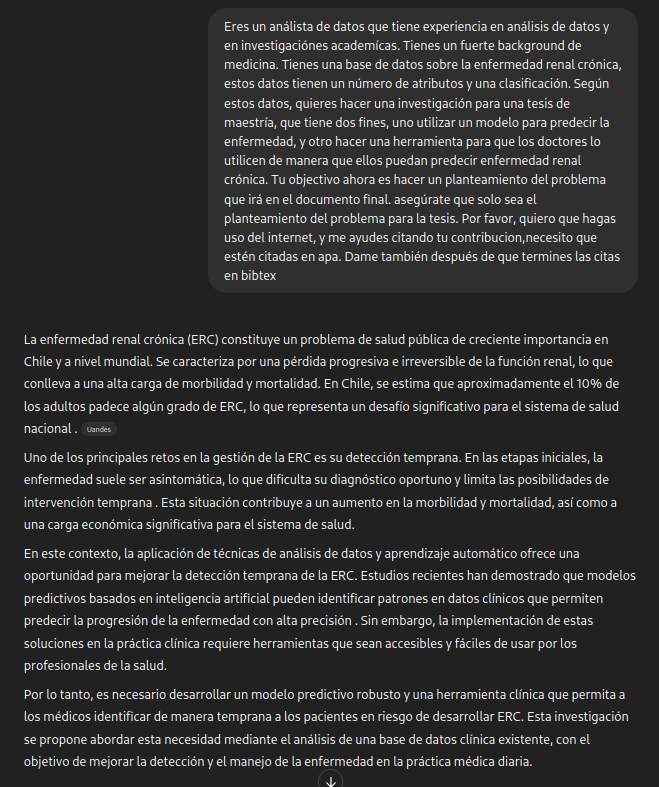
\includegraphics[width=\textwidth]{../gpt2.jpg}
\end{center}
\textbf{Citas encontradas por ChatGPT:}
\begin{itemize}
    \item Clínica Universidad de los Andes. (2023). En Chile, 10\% de los adultos tiene una enfermedad renal crónica. Recuperado de https://www.clinicauandes.cl/noticia/en-chile-10-de-los-adultos-tiene-una-enfermedad-renal-cronica
        Uandes
    \item Elsevier. (s.f.). Enfermedad renal crónica:
        epidemiología y factores de riesgo. Recuperado de
    https://www.elsevier.es/es-revista-revista-medica-clinica-las-condes-202-articulo
    -enfermedad-renal-cronica-epidemiologia-factores-S0716864010705654e
        www.elsevier.com
    \item Nefrología al Día. (2023). ARTIFICIAL: La Nueva Inteligencia y su Aplicación en Nefrología. Recuperado de https://www.nefrologiaaldia.org/es-articulo-artificial-la-nueva-inteligencia-su-609
Nefrología al Día
\end{itemize}
\newpage
\subsection{Anexo 2: Resultado Gemini primer tema}
\begin{center}
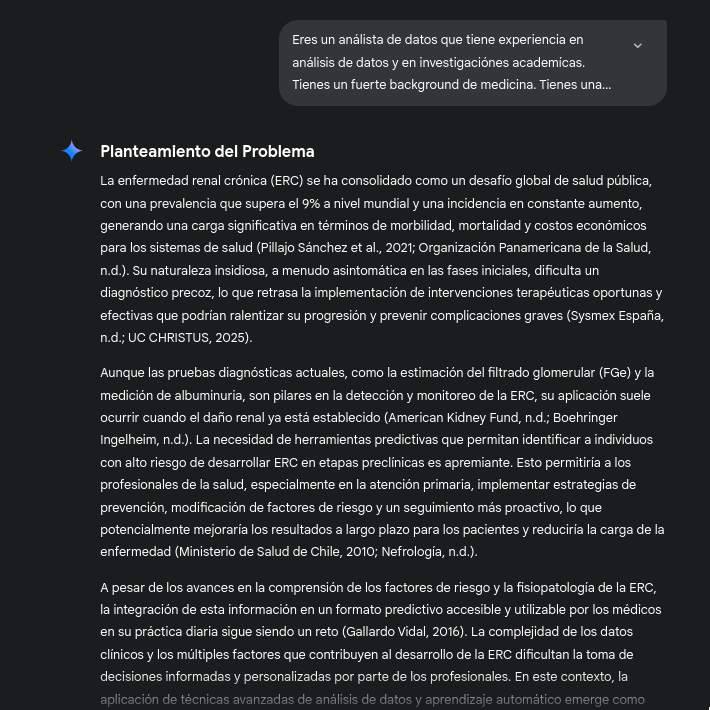
\includegraphics[width=0.8\textwidth]{../gemini1.jpg}\\
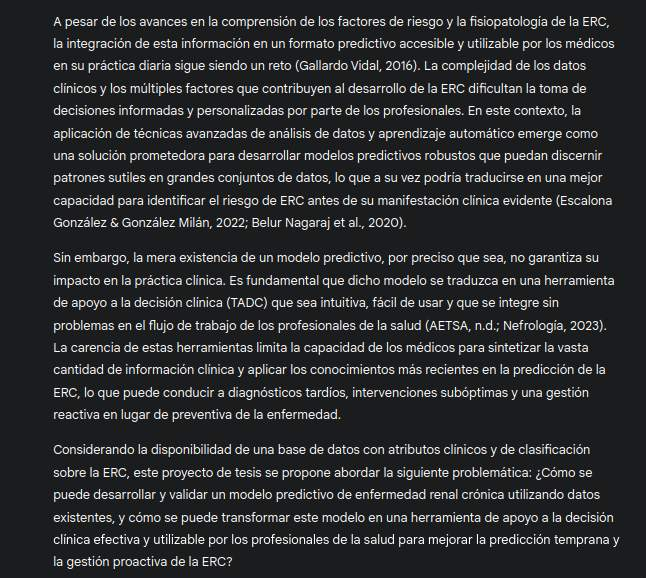
\includegraphics[width=0.8\textwidth]{../gemini2.jpg}\\
\end{center}
\textbf{Citas encontradas por Gemini}
\begin{itemize}
    \item AETSA. (n.d.). Herramienta de ayuda a la toma de decisiones de pacientes susceptibles de diálisis. Recuperado de https://www.aetsa.org/download/publicaciones/antiguas/AETSA
        \_2009-8\_HATD\_ERC.pdf
    \item American Kidney Fund. (n.d.). Las pruebas de detección de la enfermedad renal. Recuperado de https://www.kidneyfund.org/es/todo-sobre-los-rinones/las-pruebas-de-deteccion-de-la-enfermedad-renal
    \item Belur Nagaraj, S., Pena, M. J., Ju, W., \& The BEAt-DKD Consortium. (2020). Machine-learning-based early prediction of end-stage renal disease in patients with diabetic kidney disease using clinical trials data. Diabetes, 1  Obesity and Metabolism, 22(12), 2479-2486.  1. e-dmj.org e-dmj.org
    \item Boehringer Ingelheim. (n.d.). Enfermedad renal crónica: La importancia del diagnóstico temprano. Recuperado de https://www.boehringer-ingelheim.com/sa/salud-humana/enfermedad-renal-cronica/enfermedad-renal-cronica-la-importancia-del-diagnostico-temprano
    \item Escalona González, S. O., \& González Milán, Z. C. (2022). Inteligencia artificial en la predicción de mortalidad por enfermedad renal crónica. Anales de la Academia de Ciencias de Cuba, 12(3), e1292.
    \item Gallardo Vidal, L. S. (2016). Utilidad de un modelo de predicción para la enfermedad renal crónica en una unidad de primer nivel de atención. Nefrología, 36(2), 196-200.
    \item Gemini encontró muchas más citas pero ponerlas a todas no era muy util
\end{itemize}

\newpage
\subsection{Anexo 3: Resultado Claude primer tema}
\begin{center}
    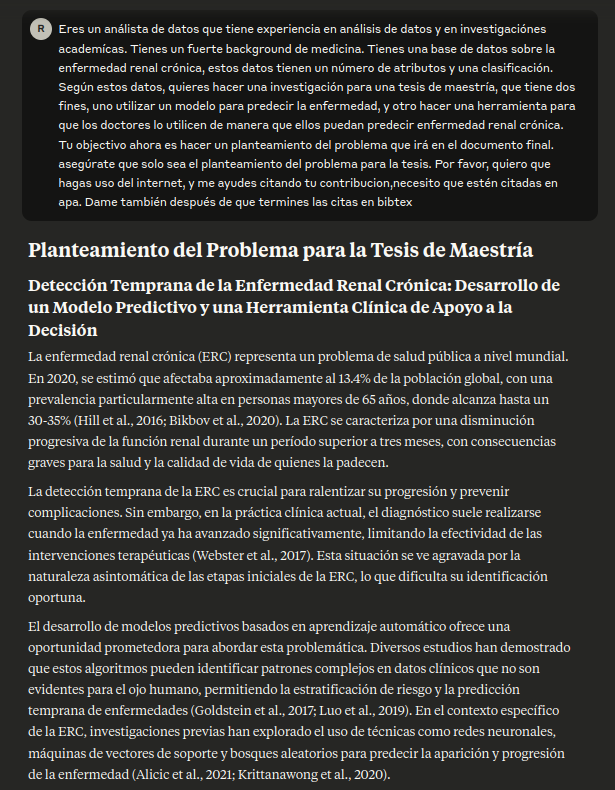
\includegraphics[width=0.6\textwidth]{../claude1.png}\\
    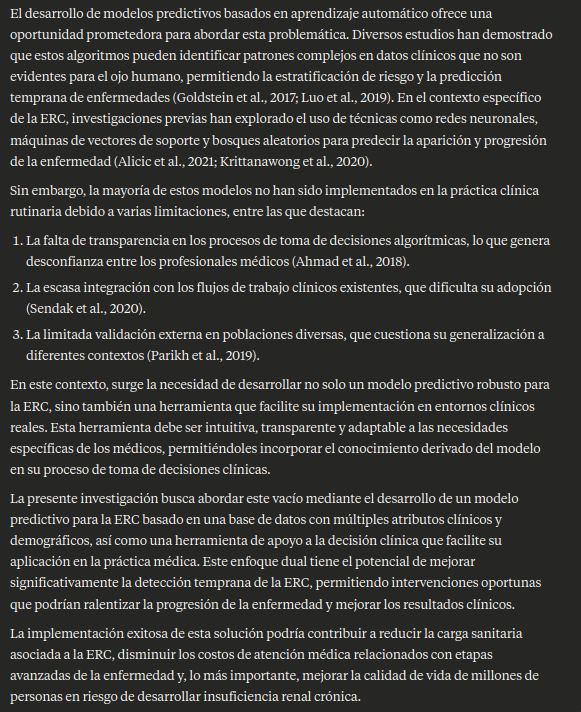
\includegraphics[width=0.6\textwidth]{../claude2.png}\\
\end{center}
\textbf{Citas encontradas por Claude}
\begin{itemize}
    \item Ahmad, M. A., Eckert, C., \& Teredesai, A. (2018). Interpretable machine learning in healthcare. Proceedings of the 2018 ACM International Conference on Bioinformatics, Computational Biology, and Health Informatics, 559-560.
    \item Alicic, R. Z., Rooney, M. T., \& Tuttle, K. R. (2021). Diabetic kidney disease: Challenges, progress, and possibilities. Clinical Journal of the American Society of Nephrology, 16(4), 423-435.
    \item Bikbov, B., Purcell, C. A., Levey, A. S., Smith, M., Abdoli, A., Abebe, M., Adebayo, O. M., Afarideh, M., Agarwal, S. K., Agudelo-Botero, M., \& others. (2020). Global, regional, and national burden of chronic kidney disease, 1990–2017: A systematic analysis for the Global Burden of Disease Study 2017. The Lancet, 395(10225), 709-733.
    \item Goldstein, B. A., Navar, A. M., \& Carter, R. E. (2017). Moving beyond regression techniques in cardiovascular risk prediction: Applying machine learning to address analytic challenges. European Heart Journal, 38(23), 1805-1814.
    \item Hill, N. R., Fatoba, S. T., Oke, J. L., Hirst, J. A., O'Callaghan, C. A., Lasserson, D. S., \& Hobbs, F. D. R. (2016). Global prevalence of chronic kidney disease – a systematic review and meta-analysis. PLoS One, 11(7), e0158765.
    \item Krittanawong, C., Virk, H. U. H., Bangalore, S., Wang, Z., Johnson, K. W., Pinotti, R., Zhang, H., Kaplin, S., Narasimhan, B., Kitai, T., \& others. (2020). Machine learning prediction in cardiovascular diseases: A meta-analysis. Scientific Reports, 10(1), 1-11.
    \item Luo, W., Phung, D., Tran, T., Gupta, S., Rana, S., Karmakar, C., Shilton, A., Yearwood, J., Dimitrova, N., Ho, T. B., \& others. (2019). Guidelines for developing and reporting machine learning predictive models in biomedical research: A multidisciplinary view. Journal of Medical Internet Research, 18(12), e323.
    \item Parikh, R. B., Teeple, S., \& Navathe, A. S. (2019). Addressing bias in artificial intelligence in health care. JAMA, 322(24), 2377-2378.
    \item Sendak, M. P., D'Arcy, J., Kashyap, S., Gao, M., Nichols, M., Corey, K., Ratliff, W., \& Balu, S. (2020). A path for translation of machine learning products into healthcare delivery. EMJ Innov, 10, 19-00172.
    \item Webster, A. C., Nagler, E. V., Morton, R. L., \& Masson, P. (2017). Chronic kidney disease. The Lancet, 389(10075), 1238-1252.
\end{itemize}
\newpage
\subsection{Anexo 4: Resultado ChatGPT segundo tema}
\begin{center}
    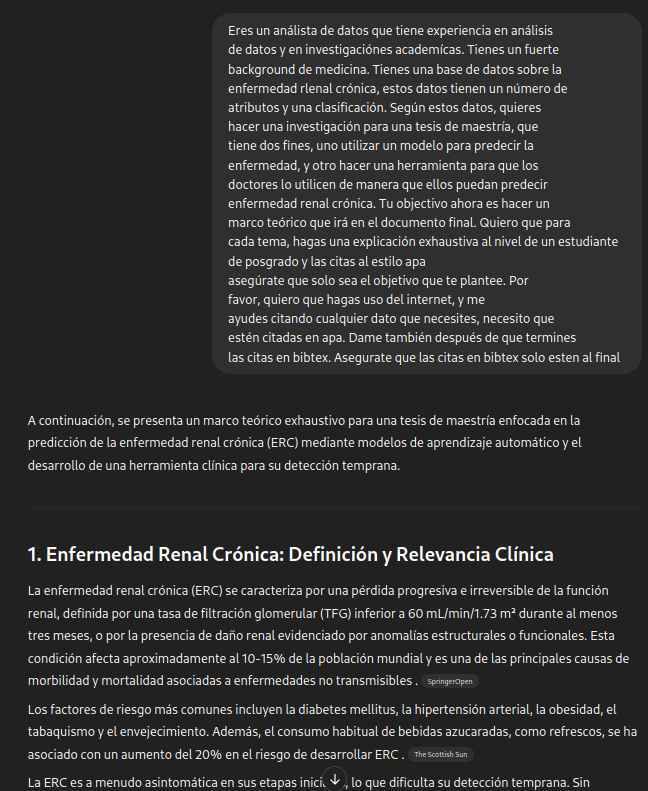
\includegraphics[width=0.6\textwidth]{../copilot_marc1.png}\\
    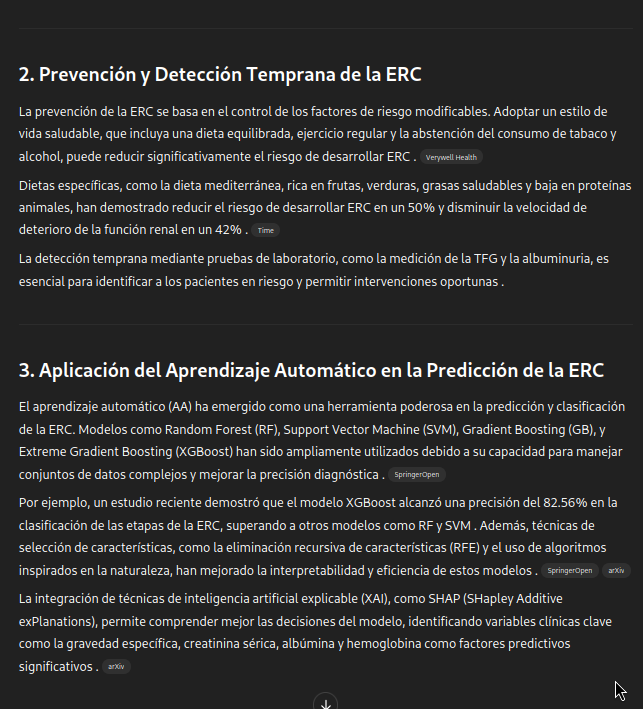
\includegraphics[width=0.6\textwidth]{../copilot_marc2.png}\\
    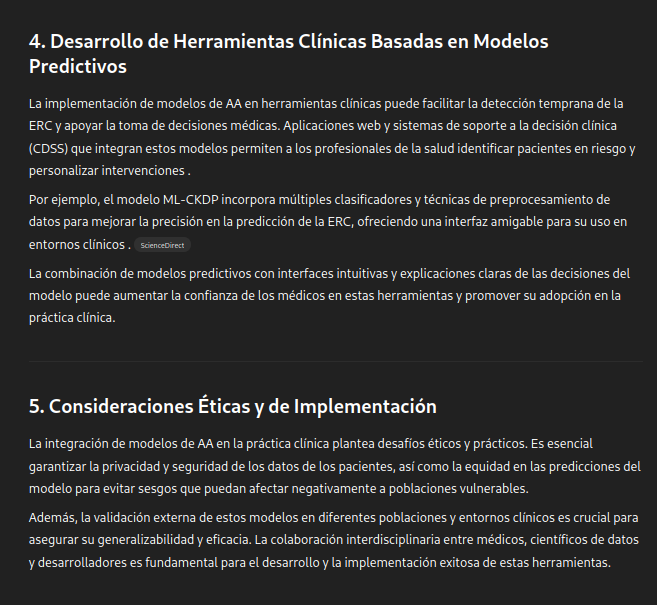
\includegraphics[width=0.6\textwidth]{../copilot_3.png}\\
\end{center}
\textbf{Citas encontradas por ChatGPT}
\begin{itemize}
    \item Belur Nagaraj, S., Pena, M. J., Ju, W., \& The BEAt-DKD Consortium. (2020). Machine-learning-based early prediction of end-stage renal disease in patients with diabetic kidney disease using clinical trials data. Diabetes, Obesity and Metabolism, 22(12), 2479-2486.
    \item Fotheringham, J., Blake, M., \& Crowe, S. (2015). Early chronic kidney disease: identification and management. Canadian Medical Association Journal, 187(18), 1339-1346.
    \item Kawamoto, K., Houlihan, C. A., Balas, E. A., \& Wyatt, J. C. (2005). Improving clinical practice: a synthesis of 16 meta-analyses of randomized controlled trials of clinical decision support systems. BMC Medical Informatics and Decision Making, 5, 4.
    \item KDIGO. (2012). KDIGO 2012 clinical practice guideline for the evaluation and management of chronic kidney disease. Kidney International Supplements, 3(1), 1-150.
    \item Levey, A. S., Eckardt, K. U., Tsukamoto, Y., Levin, A., Coresh, J., Rossert, J., ... \& Ritz, E. (2003). Definition and classification of chronic kidney disease: a position statement from Kidney Disease: Improving Global Outcomes (KDIGO). Kidney International, 67(6), 2089-2100.
    \item Lysaght, M. J. (2002). Maintenance dialysis population dynamics: current trends and long-term implications. Nephrology Dialysis Transplantation, 17(Suppl 1), 8-15.
    \item Ministerio de Salud de Chile. (2019). Encuesta Nacional de Salud 2016-2017: Primeros Resultados. Santiago: MINSAL.
    \item Romero, R. (2019). Epidemiología de la enfermedad renal crónica. Nefrología Latinoamericana, 25(1), 11-17.
    \item Tonelli, M., Wiebe, N., Culleton, B., Manns, B. J., Klarenbach, S., \& Hemmelgarn, B. R. (2006). Chronic kidney disease and mortality risk: a systematic review. Kidney International, 70(10), 1702-1710.
    \item Wuest, M., Bejnordi, B. E., \& van Ginneken, B. (2018). Machine learning for medical image analysis. Nature Medicine, 24(8), 1274-1288.
\end{itemize}
\newpage
\subsection{Anexo 5: Resultado Gemini segundo tema}
\begin{center}
    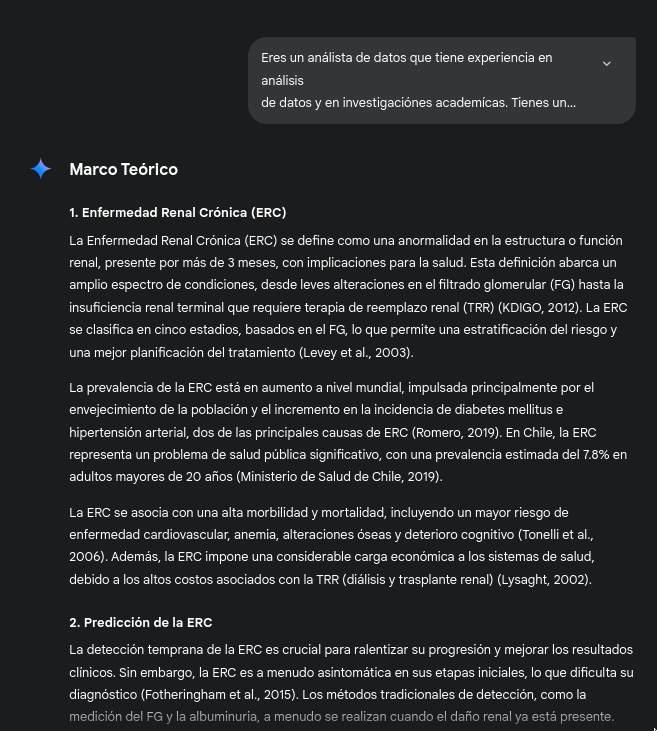
\includegraphics[width=0.6\textwidth]{../gemini_marco.png}\\
    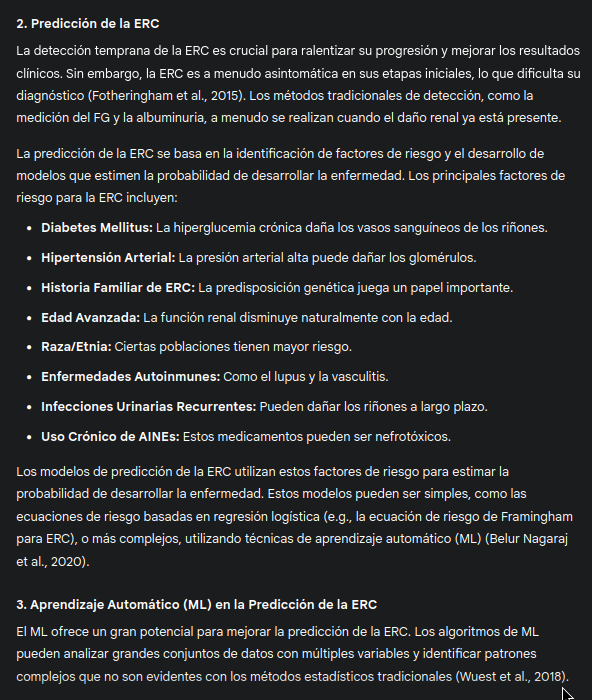
\includegraphics[width=0.6\textwidth]{../gemini_marco_2.png}\\
    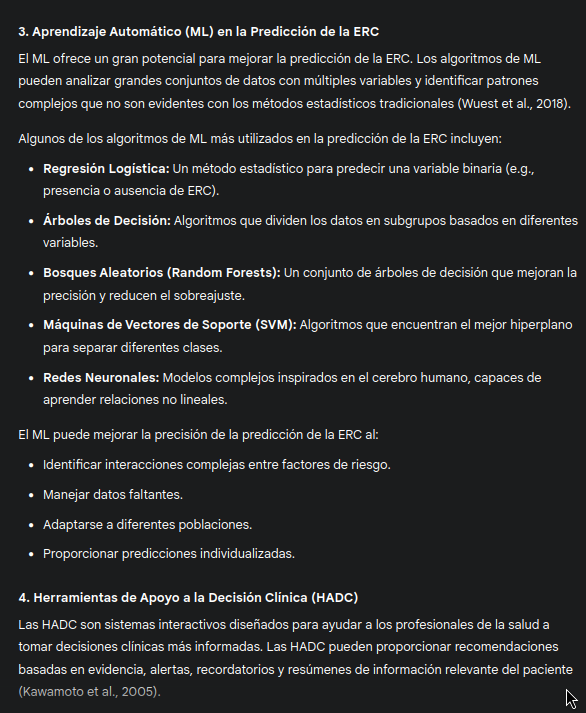
\includegraphics[width=0.6\textwidth]{../gemini3.png}\\
    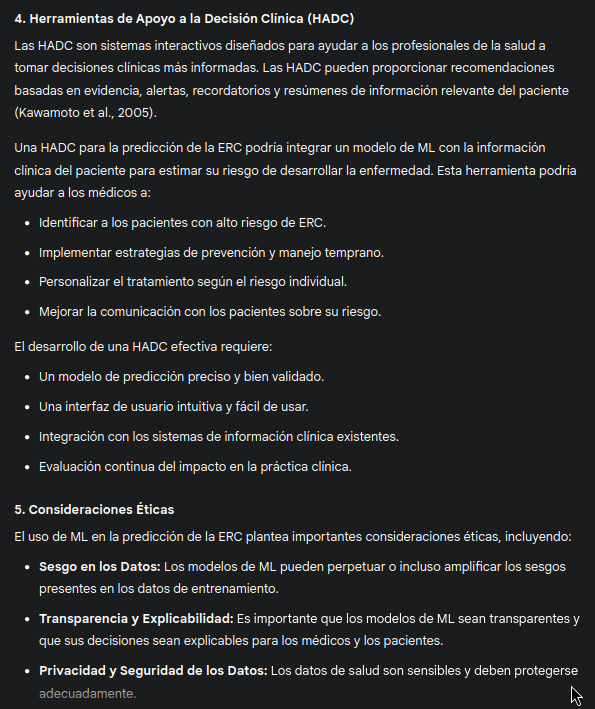
\includegraphics[width=0.6\textwidth]{../gemini_marco_4.png}\\
\end{center}
\textbf{Citas encontradas por Gemini}
\begin{itemize}
    \item Belur Nagaraj, S., Pena, M. J., Ju, W., \& The BEAt-DKD Consortium. (2020). Machine-learning-based early prediction of end-stage renal disease in patients with diabetic kidney disease using clinical trials data. Diabetes, Obesity and Metabolism, 22(12), 2479-2486.
    \item Fotheringham, J., Blake, M., \& Crowe, S. (2015). Early chronic kidney disease: identification and management. Canadian Medical Association Journal, 187(18), 1339-1346.
    \item Kawamoto, K., Houlihan, C. A., Balas, E. A., \& Wyatt, J. C. (2005). Improving clinical practice: a synthesis of 16 meta-analyses of randomized controlled trials of clinical decision support systems. BMC Medical Informatics and Decision Making, 5, 4.
    \item KDIGO. (2012). KDIGO 2012 clinical practice guideline for the evaluation and management of chronic kidney disease. Kidney International Supplements, 3(1), 1-150.
    \item Levey, A. S., Eckardt, K. U., Tsukamoto, Y., Levin, A., Coresh, J., Rossert, J., ... \& Ritz, E. (2003). Definition and classification of chronic kidney disease: a position statement from Kidney Disease: Improving Global Outcomes (KDIGO). Kidney International, 67(6), 2089-2100.
    \item Lysaght, M. J. (2002). Maintenance dialysis population dynamics: current trends and long-term implications. Nephrology Dialysis Transplantation, 17(Suppl 1), 8-15.
    \item Ministerio de Salud de Chile. (2019). Encuesta Nacional de Salud 2016-2017: Primeros Resultados. Santiago: MINSAL.
    \item Romero, R. (2019). Epidemiología de la enfermedad renal crónica. Nefrología Latinoamericana, 25(1), 11-17.
    \item Tonelli, M., Wiebe, N., Culleton, B., Manns, B. J., Klarenbach, S., \& Hemmelgarn, B. R. (2006). Chronic kidney disease and mortality risk: a systematic review. Kidney International, 70(10), 1702-1710.
    \item Wuest, M., Bejnordi, B. E., \& van Ginneken, B. (2018). Machine learning for medical image analysis. Nature Medicine, 24(8), 1274-1288.
\end{itemize}
\newpage
\subsection{Anexo 6: Resultado Claude segundo tema}
\begin{center}
    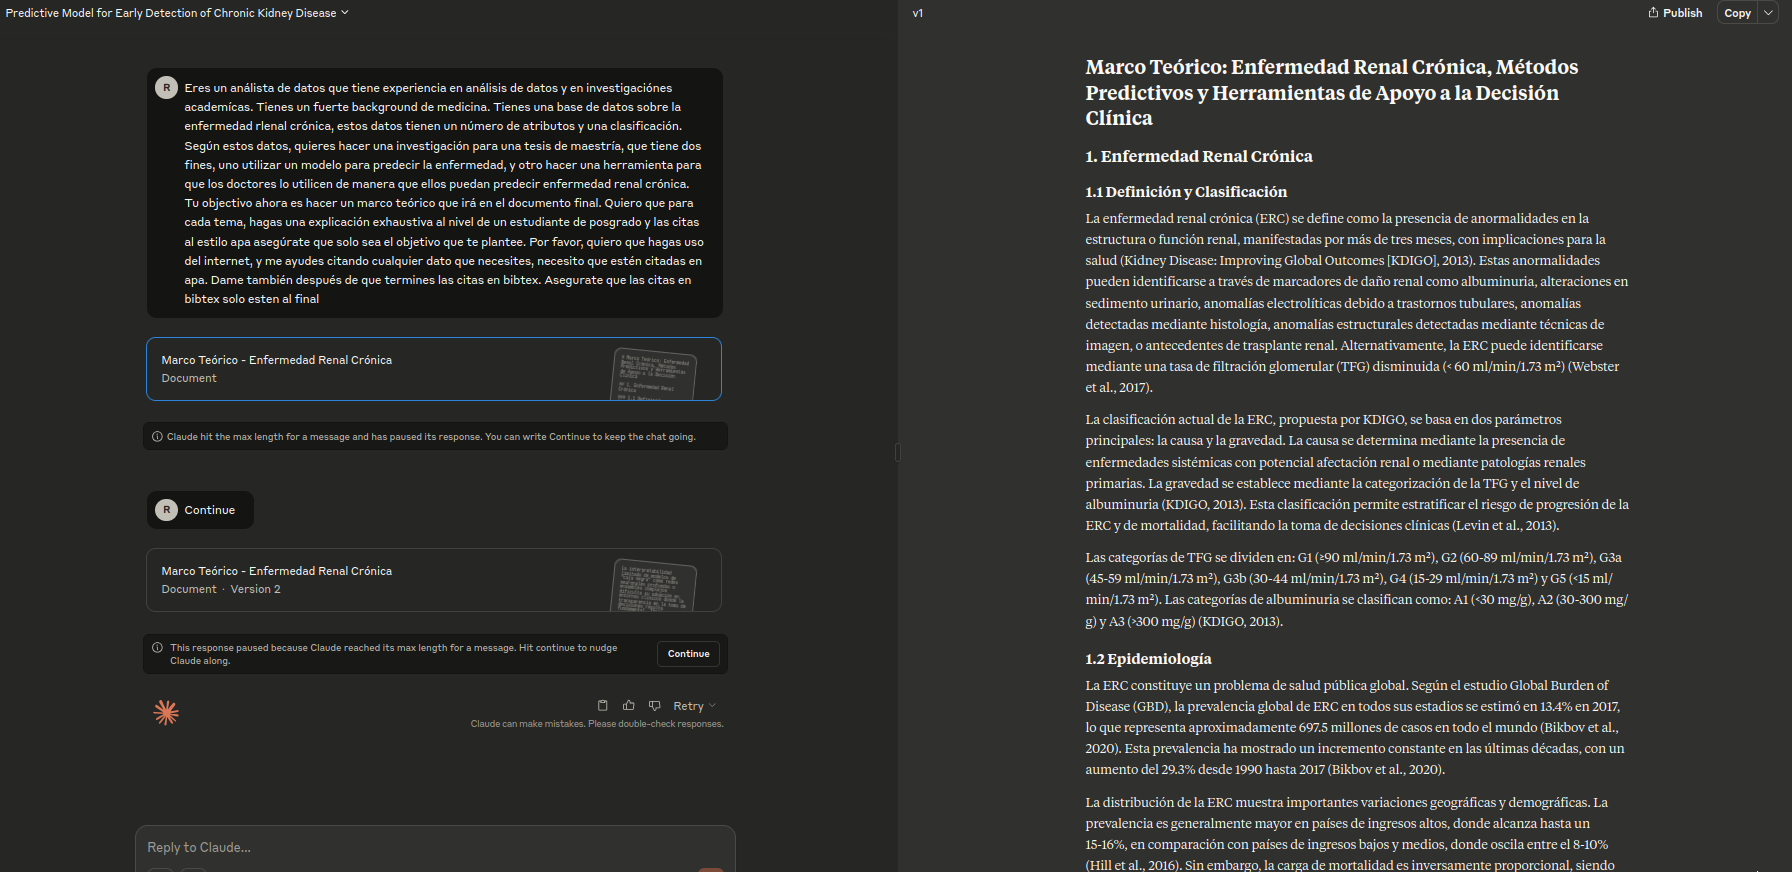
\includegraphics[width=\textwidth]{../claude_marco_1.png}\\
\end{center}
Claude me sorprendió, hizo un marco teórico completo, fue
sorprendente, tanto asi que llegó a su limite dos veces.
Presentaré el resultado no con imágenes porque es díficil de
entender, en la siguiente página esta el resultado completo de claude

\begin{itemize}
\item Webster, A. C., Nagler, E. V., Morton, R. L., \& Masson, P. (2017). Chronic kidney disease. The Lancet, 389(10075), 1238-1252. https://doi.org/10.1016/S0140-6736(16)32064-5
\item Kidney Disease: Improving Global Outcomes (KDIGO) CKD Work Group. (2013). KDIGO 2012 Clinical Practice Guideline for the Evaluation and Management of Chronic Kidney Disease. Kidney International Supplements, 3(1), 1-150.
\item Levey, A. S., \& Coresh, J. (2012). Chronic kidney disease. The Lancet, 379(9811), 165-180. https://doi.org/10.1016/S0140-6736(11)60178-5
\item GBD Chronic Kidney Disease Collaboration. (2020). Global, regional, and national burden of chronic kidney disease, 1990–2017: a systematic analysis for the Global Burden of Disease Study 2017. The Lancet, 395(10225), 709-733. https://doi.org/10.1016/S0140-6736(20)30045-3
\item Luyckx, V. A., Tonelli, M., \& Stanifer, J. W. (2018). The global burden of kidney disease and the sustainable development goals. Bulletin of the World Health Organization, 96(6), 414-422D. https://doi.org/10.2471/BLT.17.206441
\item Bikbov, B., Purcell, C. A., Levey, A. S., Smith, M., Abdoli, A., Abebe, M., ... \& Mokdad, A. H. (2020). Global, regional, and national burden of chronic kidney disease, 1990–2017: a systematic analysis for the Global Burden of Disease Study 2017. The Lancet, 395(10225), 709-733. https://doi.org/10.1016/S0140-6736(20)30045-3
\end{itemize}
\newpage
\thispagestyle{empty}
\newgeometry{bottom=25mm,hmargin=1.5cm,vmargin=2cm}
\begin{multicols}{2}
    [ \section*{Resultado de Claude}Es demaisado largo
    para dar capturas]
\tiny Marco Teórico: Enfermedad Renal Crónica, Métodos Predictivos y Herramientas de Apoyo a la Decisión Clínicahh
 1. Enfermedad Renal Crónica
 1.1 Definición y Clasificación
La enfermedad renal crónica (ERC) se define como la presencia de anormalidades en la estructura o función renal, manifestadas por más de tres meses, con implicaciones para la salud (Kidney Disease: Improving Global Outcomes [KDIGO], 2013). Estas anormalidades pueden identificarse a través de marcadores de daño renal como albuminuria, alteraciones en sedimento urinario, anomalías electrolíticas debido a trastornos tubulares, anomalías detectadas mediante histología, anomalías estructurales detectadas mediante técnicas de imagen, o antecedentes de trasplante renal. Alternativamente, la ERC puede identificarse mediante una tasa de filtración glomerular (TFG) disminuida (< 60 ml/min/1.73 m²) (Webster et al., 2017).
La clasificación actual de la ERC, propuesta por KDIGO, se basa en dos parámetros principales: la causa y la gravedad. La causa se determina mediante la presencia de enfermedades sistémicas con potencial afectación renal o mediante patologías renales primarias. La gravedad se establece mediante la categorización de la TFG y el nivel de albuminuria (KDIGO, 2013). Esta clasificación permite estratificar el riesgo de progresión de la ERC y de mortalidad, facilitando la toma de decisiones clínicas (Levin et al., 2013).
Las categorías de TFG se dividen en: G1 (>90 ml/min/1.73 m²), G2 (60-89 ml/min/1.73 m²), G3a (45-59 ml/min/1.73 m²), G3b (30-44 ml/min/1.73 m²), G4 (15-29 ml/min/1.73 m²) y G5 (<15 ml/min/1.73 m²). Las categorías de albuminuria se clasifican como: A1 (<30 mg/g), A2 (30-300 mg/g) y A3 (>300 mg/g) (KDIGO, 2013).
 1.2 Epidemiología
La ERC constituye un problema de salud pública global. Según el estudio Global Burden of Disease (GBD), la prevalencia global de ERC en todos sus estadios se estimó en 13.4% en 2017, lo que representa aproximadamente 697.5 millones de casos en todo el mundo (Bikbov et al., 2020). Esta prevalencia ha mostrado un incremento constante en las últimas décadas, con un aumento del 29.3% desde 1990 hasta 2017 (Bikbov et al., 2020).
La distribución de la ERC muestra importantes variaciones geográficas y demográficas. La prevalencia es generalmente mayor en países de ingresos altos, donde alcanza hasta un 15-16%, en comparación con países de ingresos bajos y medios, donde oscila entre el 8-10% (Hill et al., 2016). Sin embargo, la carga de mortalidad es inversamente proporcional, siendo más elevada en regiones de África subsahariana, Asia meridional y Oceanía, reflejando disparidades en el acceso a servicios de salud (Bikbov et al., 2020).
En términos demográficos, la prevalencia de ERC aumenta significativamente con la edad, afectando aproximadamente al 30-35% de los individuos mayores de 65 años en comparación con el 5-7% en adultos jóvenes (Glassock et al., 2017). El sexo femenino presenta una mayor prevalencia de ERC en estadios tempranos, mientras que el sexo masculino muestra mayor progresión hacia estadios avanzados (Ricardo et al., 2019).
 1.3 Factores de Riesgo
Los factores de riesgo para el desarrollo y progresión de la ERC pueden categorizarse como no modificables y modificables. Entre los factores no modificables destacan la edad avanzada, el sexo masculino, la raza (particularmente afroamericana e hispana), la historia familiar de enfermedad renal y la predisposición genética, incluidos los polimorfismos en genes como APOL1, UMOD y MYH9 (Genovese et al., 2018; Parsa et al., 2013).
Los factores de riesgo modificables incluyen enfermedades sistémicas como la diabetes mellitus y la hipertensión arterial, que juntas constituyen aproximadamente el 70% de las causas de ERC terminal en países desarrollados (Tuttle et al., 2014). La obesidad, definida como un índice de masa corporal ≥30 kg/m², representa un factor de riesgo independiente para el desarrollo de ERC, tanto directamente a través de la glomerulopatía asociada a la obesidad como indirectamente mediante la promoción de resistencia a la insulina y síndrome metabólico (Kovesdy et al., 2017).
Otros factores de riesgo modificables incluyen el tabaquismo, que acelera la progresión de la ERC a través de mecanismos como la disfunción endotelial y el estrés oxidativo (Orth \& Hallan, 2008); la exposición a nefrotoxinas, incluidos ciertos medicamentos como antiinflamatorios no esteroideos y contrastes radiológicos; y factores socioeconómicos como el nivel educativo bajo y el acceso limitado a servicios de salud (Morton et al., 2016).
 1.4 Fisiopatología
La fisiopatología de la ERC es compleja y multifactorial, involucrando mecanismos adaptativos iniciales que eventualmente se vuelven maladaptativos. Independientemente de la etiología inicial, la pérdida de nefronas funcionales conduce a una serie de cambios hemodinámicos, metabólicos e inflamatorios que establecen un ciclo de daño renal progresivo (Schlondorff, 2008).
La hiperfiltración glomerular representa uno de los mecanismos centrales en la progresión de la ERC. Cuando se pierde un número crítico de nefronas, las nefronas restantes compensan aumentando su tasa de filtración individual, lo que conlleva un incremento de la presión intraglomerular. Este fenómeno, descrito por Brenner como la "hipótesis de la hiperfiltración", conduce a esclerosis glomerular y pérdida adicional de nefronas, estableciendo un círculo vicioso (Brenner et al., 1996).
Los cambios estructurales característicos incluyen
glomeruloesclerosis, atrofia tubular, fibrosis intersticial
e inflamación crónica. A nivel molecular, la activación del
sistema renina-angiotensina-aldosterona (SRAA) juega un
papel crucial, promoviendo vasoconstricción, retención de
sodio, hipertensión intraglomerular y liberación de
citoquinas profibróticas como el factor de crecimiento
transformante beta (TGF-B) (Remuzzi et al., 2006).
Los procesos inflamatorios crónicos están mediados por la
activación de células inmunes residentes y reclutadas, que
producen citoquinas proinflamatorias como IL-1, IL-6 y
TNF-A. Estas citoquinas, junto con factores de crecimiento
como el PDGF y el TGF-B, promueven la transdiferenciación de
células tubulares epiteliales a miofibroblastos, un proceso
conocido como transición epitelio-mesénquima, que contribuye
significativamente a la fibrosis renal (Liu, 2011).
El estrés oxidativo, caracterizado por un desequilibrio
entre la producción de especies reactivas de oxígeno (ROS) y
los mecanismos antioxidantes, representa otro mecanismo
patogénico relevante. Los ROS causan daño directo a lípidos,
proteínas y ADN celular, además de activar vías de
señalización que promueven inflamación y fibrosis (Ruiz et
al., 2013).
 1.5 Manifestaciones Clínicas y Complicaciones
Las manifestaciones clínicas de la ERC varían según el estadio de la enfermedad, la etiología subyacente y la presencia de comorbilidades. Los estadios iniciales (G1-G3a) suelen ser asintomáticos, detectándose frecuentemente mediante hallazgos incidentales en análisis rutinarios (Webster et al., 2017).
A medida que la función renal se deteriora (estadios G3b-G5), pueden aparecer síntomas inespecíficos como fatiga, anorexia, náuseas, prurito y alteraciones del sueño. Las complicaciones específicas de la ERC incluyen la anemia, principalmente debido a la disminución en la producción de eritropoyetina; alteraciones del metabolismo mineral y óseo, que conducen a la osteodistrofia renal; acidosis metabólica, resultante de la disminución en la excreción de ácidos; y desnutrición proteico-calórica, característica del síndrome de desgaste asociado a la ERC (Kazancioğlu, 2013).
Las complicaciones cardiovasculares representan la principal causa de morbimortalidad en pacientes con ERC. La asociación entre ERC y enfermedad cardiovascular es bidireccional: la ERC constituye un factor de riesgo independiente para eventos cardiovasculares, mientras que la enfermedad cardiovascular puede acelerar la progresión de la ERC. Los mecanismos implicados incluyen la calcificación vascular acelerada, disfunción endotelial, inflamación crónica, estrés oxidativo y activación simpática (Go et al., 2004; Sarnak et al., 2003).
Las complicaciones neurológicas abarcan desde la encefalopatía urémica en estadios avanzados hasta alteraciones cognitivas sutiles en estadios tempranos. La neuropatía periférica, caracterizada por polineuropatía sensoriomotora simétrica distal, afecta hasta al 60-100% de los pacientes en diálisis (Krishnan \& Kiernan, 2009).
Las alteraciones hidroelectrolíticas y del equilibrio ácido-base son frecuentes en la ERC avanzada e incluyen hiperpotasemia, hiponatremia, hiperfosfatemia, hipocalcemia y acidosis metabólica, cada una con sus manifestaciones clínicas específicas y potenciales complicaciones (Palmer \& Clegg, 2015).
 1.6 Diagnóstico y Evaluación
El diagnóstico de la ERC se basa en la detección de anomalías estructurales o funcionales del riñón que persisten durante más de tres meses. La evaluación inicial debe incluir la historia clínica completa, exploración física, análisis de orina, determinaciones bioquímicas séricas y estudios de imagen (KDIGO, 2013).
La TFG constituye el mejor indicador global de la función renal. Aunque la medición directa mediante aclaramiento de inulina representa el estándar de oro, en la práctica clínica se utilizan ecuaciones predictivas basadas en la creatinina sérica, como la ecuación CKD-EPI (Chronic Kidney Disease Epidemiology Collaboration), que ha demostrado mayor precisión que fórmulas previas como MDRD (Modification of Diet in Renal Disease) (Levey et al., 2009). Recientemente, biomarcadores alternativos como la cistatina C han mostrado utilidad complementaria, especialmente en poblaciones específicas como ancianos, pacientes con masa muscular reducida o con función renal entre normal y levemente reducida (Inker et al., 2012).
La evaluación de la albuminuria, preferentemente mediante el cociente albúmina/creatinina en una muestra aislada de orina, constituye un indicador sensible de daño glomerular y un predictor independiente de progresión de la ERC y de eventos cardiovasculares (Hemmelgarn et al., 2010).
Los estudios de imagen, particularmente la ecografía renal, permiten evaluar la morfología y tamaño renales, detectar obstrucción de la vía urinaria y valorar la presencia de lesiones quísticas o masas renales. Técnicas avanzadas como la resonancia magnética, especialmente secuencias funcionales como la difusión, elastografía o la espectroscopia, ofrecen información adicional sobre fibrosis y microestructura renal (Grenier et al., 2016).
La biopsia renal permanece como el método diagnóstico definitivo para determinar la etiología específica de muchas nefropatías, especialmente en casos de proteinuria significativa, hematuria glomerular, deterioro inexplicado de la función renal o sospecha de enfermedades sistémicas con afectación renal (Fiorentino et al., 2016).
 1.7 Tratamiento y Manejo
El manejo de la ERC debe ser integral, adaptado al estadio de la enfermedad y a las comorbilidades del paciente. Los objetivos terapéuticos incluyen la ralentización de la progresión de la enfermedad, la prevención y tratamiento de complicaciones, y la preparación adecuada para la terapia renal sustitutiva cuando sea necesaria (KDIGO, 2013).
Las intervenciones para retrasar la progresión de la ERC incluyen el control estricto de la presión arterial, con objetivos específicos según el perfil de riesgo del paciente y el grado de albuminuria. Los inhibidores del sistema renina-angiotensina-aldosterona, como los inhibidores de la enzima convertidora de angiotensina (IECA) y los antagonistas de los receptores de angiotensina II (ARA-II), constituyen la primera línea terapéutica por su efecto nefroprotector adicional, independiente de la reducción de la presión arterial (Ruggenenti et al., 2012). Los inhibidores del cotransportador sodio-glucosa tipo 2 (iSGLT2) y los agonistas del receptor del péptido similar al glucagón tipo 1 (arGLP-1) han emergido como opciones terapéuticas prometedoras en pacientes con ERC, especialmente aquellos con diabetes mellitus tipo 2, debido a sus efectos renoprotectores demostrados en ensayos clínicos recientes (Perkovic et al., 2019; Mann et al., 2017).
El control glucémico óptimo en pacientes diabéticos es esencial para la prevención y manejo de la nefropatía diabética. La hemoglobina glicosilada objetivo debe individualizarse según la edad del paciente, comorbilidades, riesgo de hipoglucemia y expectativa de vida (Tuttle et al., 2014).
Las modificaciones dietéticas incluyen la restricción proteica moderada (0.6-0.8 g/kg/día), que ha demostrado ralentizar la progresión de la ERC en algunos estudios, aunque la evidencia no es concluyente. La restricción de sodio (<2 g/día), la moderación en la ingesta de potasio y fósforo, y la adecuada ingesta calórica son otros aspectos dietéticos relevantes (Kalantar-Zadeh \& Fouque, 2017).
El manejo de las complicaciones específicas incluye la
corrección de la anemia mediante agentes estimuladores de la
eritropoyesis y suplementos de hierro; el tratamiento de las
alteraciones del metabolismo mineral y óseo mediante
quelantes del fósforo, análogos de la vitamina D y
calcimiméticos; la corrección de la acidosis metabólica
mediante suplementos de bicarbonato; y el manejo del prurito
mediante emolientes tópicos, gabapentinoides y, en casos
refractarios, antagonistas del receptor u-opioide (Palmer et
al., 2013; Bover et al., 2019).
La terapia renal sustitutiva, que incluye la diálisis (hemodiálisis o diálisis peritoneal) y el trasplante renal, está indicada en estadios avanzados de ERC (TFG <15 ml/min/1.73 m²) o antes si existen síntomas o complicaciones urémicas. El trasplante renal, cuando es posible, ofrece la mejor supervivencia y calidad de vida a largo plazo (Wolfe et al., 1999).
Los cuidados paliativos deben integrarse precozmente en el manejo de pacientes con ERC avanzada, especialmente en aquellos con múltiples comorbilidades, edad avanzada o contraindicaciones para terapia renal sustitutiva, enfocándose en el control de síntomas y la mejora de la calidad de vida (Davison, 2011).
 2. Modelos Predictivos en Salud
 2.1 Fundamentos del Aprendizaje Automático en Medicina
El aprendizaje automático (Machine Learning, ML) representa un subconjunto de la inteligencia artificial que desarrolla algoritmos capaces de aprender patrones a partir de datos, sin ser explícitamente programados para tareas específicas. En el contexto médico, estos algoritmos pueden extraer relaciones complejas entre variables clínicas, genéticas, demográficas y ambientales para predecir diagnósticos, pronósticos o respuestas terapéuticas (Rajkomar et al., 2019).
Los paradigmas fundamentales del aprendizaje automático incluyen el aprendizaje supervisado, donde los algoritmos aprenden a partir de ejemplos etiquetados; el aprendizaje no supervisado, que identifica patrones intrínsecos en datos no etiquetados; y el aprendizaje por refuerzo, que optimiza decisiones secuenciales a través de sistemas de recompensa (Deo, 2015).
Las aplicaciones del ML en medicina abarcan desde la interpretación automatizada de imágenes diagnósticas hasta la predicción de reingresos hospitalarios, la estratificación de riesgo de enfermedades y la medicina de precisión (Beam \& Kohane, 2018). La integración de estas tecnologías promete transformar el paradigma médico actual hacia un modelo predictivo, preventivo, personalizado y participativo (medicina 4P) (Hood \& Friend, 2011).
A pesar de su potencial, la implementación del ML en la práctica clínica enfrenta desafíos significativos, incluidos la calidad y representatividad de los datos, la reproducibilidad de los modelos, la interpretabilidad algoritmica y las consideraciones éticas y regulatorias (Shah et al., 2019).
 2.2 Tipos de Algoritmos y su Aplicación en Nefrología
Diversos algoritmos de aprendizaje automático han sido aplicados en el contexto de la nefrología, cada uno con características específicas que los hacen más adecuados para determinados tipos de problemas y conjuntos de datos.
Los modelos de regresión logística, aunque técnicamente no se consideran algoritmos de aprendizaje automático avanzados, representan el punto de partida para la mayoría de análisis predictivos en nefrología debido a su interpretabilidad y relativa simplicidad. Estos modelos han sido ampliamente utilizados para la predicción del riesgo de ERC en poblaciones de alto riesgo (Tangri et al., 2011).
Las máquinas de vectores de soporte (Support Vector Machines, SVM) son métodos de clasificación que buscan el hiperplano que mejor separa las clases en un espacio multidimensional. En nefrología, han demostrado utilidad en la clasificación de biopsias renales a partir de imágenes microscópicas y en la predicción de la progresión de la ERC (Nellore \& Thompson, 2018).
Los árboles de decisión y sus extensiones como Random Forest y Gradient Boosting representan algoritmos particularmente valiosos en el contexto clínico debido a su capacidad para manejar datos heterogéneos y su interpretabilidad relativa. Estos modelos han sido aplicados para la predicción de la progresión de la ERC, la identificación de pacientes con riesgo de lesión renal aguda y la estratificación del riesgo en pacientes con trasplante renal (Leung et al., 2013; Lee et al., 2018).
Las redes neuronales artificiales, especialmente las arquitecturas profundas (Deep Learning), han revolucionado la capacidad de procesamiento de datos complejos como imágenes, señales y texto no estructurado. En nefrología, se han aplicado para la segmentación automática de riñones en imágenes radiológicas, la interpretación automatizada de biopsias renales y la predicción de la progresión de la ERC integrando múltiples fuentes de datos (Kuo et al., 2019).
Los modelos bayesianos, basados en el teorema de Bayes, incorporan conocimiento previo y cuantifican explícitamente la incertidumbre en sus predicciones, características particularmente valiosas en la toma de decisiones clínicas. Estos modelos han sido utilizados para la predicción de eventos adversos en pacientes con ERC y para la personalización de regímenes de diálisis (Ibrahim et al., 2019).
 2.3 Desarrollo y Validación de Modelos Predictivos
El desarrollo de modelos predictivos robustos requiere una metodología rigurosa que comprende múltiples etapas, desde la definición del problema hasta la implementación y monitorización en entornos clínicos reales.
La definición del problema clínico constituye el punto de partida, especificando claramente la población objetivo, el resultado a predecir, el horizonte temporal de la predicción y la utilidad clínica esperada del modelo. Esta fase debe involucrar a expertos clínicos para garantizar la relevancia y aplicabilidad del modelo (Steyerberg \& Vergouwe, 2014).
La selección y preparación de datos representa un paso crítico. Los conjuntos de datos deben ser representativos de la población objetivo y contener variables predictoras relevantes con calidad adecuada. El preprocesamiento de datos incluye la gestión de valores ausentes, la normalización de variables continuas, la codificación de variables categóricas y la detección y manejo de valores atípicos (Kuhn \& Johnson, 2013).
La selección de características (feature selection) busca identificar el subconjunto óptimo de variables predictoras, eliminando aquellas redundantes o irrelevantes. Este proceso mejora la generalización del modelo, reduce la dimensionalidad y facilita la interpretación. Métodos comunes incluyen enfoques basados en filtros (correlación, información mutua), enfoques basados en modelos (regularización Lasso, Ridge) y métodos de envoltura (wrapper methods) (Guyon \& Elisseeff, 2003).
El entrenamiento del modelo implica la optimización de hiperparámetros específicos del algoritmo seleccionado. Técnicas como la validación cruzada y la búsqueda en rejilla (grid search) permiten identificar la configuración óptima que maximiza el rendimiento sin sobreajuste (Luo et al., 2016).
La evaluación del rendimiento debe realizarse en conjuntos de datos independientes no utilizados durante el entrenamiento. Métricas comunes incluyen el área bajo la curva ROC (AUC-ROC), sensibilidad, especificidad, valor predictivo positivo y negativo, y el estadístico C (concordancia). Para modelos de regresión, se utilizan métricas como el error cuadrático medio (RMSE) y el coeficiente de determinación (R²) (Alba et al., 2017).
La calibración del modelo evalúa la concordancia entre las probabilidades predichas y las frecuencias observadas del evento. Se visualiza mediante gráficos de calibración y se cuantifica con estadísticos como la prueba de Hosmer-Lemeshow o el índice de calibración (Steyerberg et al., 2010).
La validación externa en cohortes independientes, preferiblemente de diferentes instituciones o periodos temporales, resulta esencial para evaluar la generalización del modelo a nuevas poblaciones. La discriminación y calibración pueden deteriorarse significativamente en la validación externa, lo que subraya la importancia de este paso (Siontis et al., 2015).
La interpretabilidad del modelo cobra especial relevancia en el contexto médico. Técnicas como SHAP (SHapley Additive exPlanations) y LIME (Local Interpretable Model-agnostic Explanations) permiten comprender las contribuciones individuales de cada variable a las predicciones específicas, facilitando la aceptación por parte de los profesionales clínicos (Lundberg \& Lee, 2017).
La evaluación del impacto clínico mediante estudios de implementación representa la validación definitiva de un modelo predictivo. Estos estudios evalúan si la implementación del modelo en la práctica clínica mejora los resultados de los pacientes, la eficiencia de los procesos asistenciales o la relación coste-efectividad (Moons et al., 2012).
 2.4 Modelos Específicos para Predicción de ERC
La literatura científica recoge numerosos modelos predictivos específicamente desarrollados para la identificación temprana de la ERC, la predicción de su progresión o la estimación del riesgo de complicaciones asociadas.
El modelo de Tangri, también conocido como Kidney Failure Risk Equation (KFRE), representa uno de los modelos más validados para la predicción de la progresión a enfermedad renal terminal en pacientes con ERC. Desarrollado inicialmente en una cohorte canadiense y posteriormente validado en múltiples poblaciones internacionales, este modelo integra variables clínicas y de laboratorio fácilmente disponibles como edad, sexo, TFG estimada, albuminuria, calcio sérico, fósforo, bicarbonato y albúmina. Existen versiones de 4 y 8 variables con rendimiento similar, lo que facilita su aplicación en diferentes contextos clínicos (Tangri et al., 2011; Tangri et al., 2016).
El modelo QKidney, desarrollado en el Reino Unido a partir de registros electrónicos de atención primaria, estima el riesgo de desarrollar ERC moderada-severa a 5 años en población general. Incorpora factores demográficos, comorbilidades, medicaciones y factores de riesgo modificables como tabaquismo e índice de masa corporal. Destaca por su desarrollo en una amplia muestra poblacional (más de 2.5 millones de individuos) y su integración en calculadoras clínicas de uso rutinario en atención primaria (Hippisley-Cox \& Coupland, 2010).
El modelo de Johns Hopkins para la identificación de ERC no diagnosticada utiliza datos administrativos y demográficos para identificar individuos con alta probabilidad de ERC no reconocida en entornos de atención primaria. Este enfoque permite la detección oportunista de casos sin necesidad de pruebas adicionales, maximizando la eficiencia del cribado (Chang et al., 2019).
En el ámbito de la lesión renal aguda (LRA) como precursora de ERC, el modelo AKI to CKD integra características de episodios de LRA (duración, severidad, recurrencia) con marcadores tradicionales de riesgo renal para predecir el desarrollo posterior de ERC. Este modelo subraya la importancia del seguimiento nefrológico post-LRA (Chawla et al., 2017).
Los modelos basados en aprendizaje automático avanzado para la predicción de ERC han proliferado en los últimos años. Chen et al. (2019) desarrollaron un modelo basado en redes neuronales profundas que integra datos longitudinales de historias clínicas electrónicas, demostrando superior rendimiento predictivo comparado con modelos estadísticos tradicionales. Koyner et al. (2018) aplicaron algoritmos de gradient boosting para la predicción temprana de ERC incidente a partir de datos rutinarios de laboratorio, alcanzando valores de AUC superiores a 0.90.
Los modelos específicos para poblaciones especiales incluyen el modelo SCORED para población diabética, que estratifica el riesgo de ERC en pacientes con diabetes mellitus tipo 2 utilizando variables simples como edad, índice de masa corporal, antecedentes cardiovasculares y parámetros analíticos básicos (Bang et al., 2007), y el modelo CRIC para pacientes con ERC establecida, que predice la progresión de la enfermedad incorporando biomarcadores específicos de lesión tubular como KIM-1 y NGAL (Bansal et al., 2016).
 2.5 Evaluación del Rendimiento y Limitaciones
La evaluación rigurosa del rendimiento de los modelos predictivos resulta esencial para determinar su validez y utilidad clínica. Esta evaluación debe considerar múltiples dimensiones y reconocer las limitaciones inherentes a los datos y algoritmos utilizados.
La discriminación, que evalúa la capacidad del modelo para distinguir entre individuos que experimentarán y no experimentarán el evento de interés, se cuantifica habitualmente mediante el estadístico C o área bajo la curva ROC (AUC-ROC). Valores superiores a 0.8 se consideran indicativos de buena discriminación, aunque este umbral puede variar según el contexto clínico y la prevalencia del evento (Alba et al., 2017).
La calibración, que evalúa la concordancia entre las probabilidades predichas y las frecuencias observadas del evento, resulta crítica para la toma de decisiones individualizadas. Se visualiza mediante gráficos de calibración que comparan probabilidades predichas y observadas en deciles de riesgo, y se cuantifica mediante pruebas estadísticas como Hosmer-Lemeshow o índices de recalibración (Van Calster et al., 2019).
La utilidad clínica trasciende medidas puramente estadísticas para evaluar el beneficio neto de utilizar el modelo en la práctica clínica. El análisis de curvas de decisión (decision curve analysis) representa una metodología clave para cuantificar este beneficio a diferentes umbrales de decisión clínica, incorporando las consecuencias relativas de falsos positivos y negativos (Vickers et al., 2016).
Entre las limitaciones comunes de los modelos predictivos en nefrología destacan el sesgo de selección en las cohortes de desarrollo, particularmente la infrarrepresentación de minorías étnicas y poblaciones socioeconómicamente desfavorecidas; la variabilidad en la definición de desenlaces, especialmente relevante en ERC donde diferentes criterios de progresión dificultan la comparabilidad entre estudios; y el manejo inadecuado de datos longitudinales, que frecuentemente ignora la naturaleza dinámica de factores de riesgo y biomarcadores (He et al., 2019).
El sobreajuste (overfitting) representa una limitación particularmente relevante en modelos complejos con múltiples variables predictoras y tamaños muestrales limitados. Este fenómeno conduce a excelente rendimiento en datos de entrenamiento pero pobre generalización a nuevas cohortes. Técnicas como regularización, validación cruzada y conjuntos de prueba independientes ayudan a mitigar este problema (Riley et al., 2019).
La interpretabilidad limitada de modelos de "caja negra" como redes neuronales profundas o ensambles complejos dificulta su adopción en entornos clínicos donde la transparencia en la toma de decisiones resulta fundamental. Técnicas emergentes de interpretabilidad como SHAP, LIME y análisis de importancia de características intentan abordar esta limitación, aunque a menudo a expensas de la precisión o la complejidad computacional (Ahmad et al., 2018).
La generalización limitada a nuevas poblaciones o entornos clínicos constituye un desafío persistente. Modelos desarrollados en poblaciones específicas pueden mostrar rendimiento subóptimo cuando se aplican a pacientes de diferentes características demográficas, con patrones de comorbilidad distintos o atendidos en sistemas sanitarios con prácticas divergentes. La transferencia de aprendizaje y la actualización adaptativa de modelos representan estrategias prometedoras para abordar esta limitación (Wiens et al., 2019).
La disponibilidad y calidad de datos en tiempo real para la implementación clínica representa otro obstáculo significativo. Muchos modelos se desarrollan con datos retrospectivos cuidadosamente curados, pero deben enfrentarse en la implementación a datos incompletos, inconsistentes o registrados con diferentes estándares y definiciones (Chen \& Asch, 2017).
 3. Herramientas de Apoyo a la Decisión Clínica
 3.1 Definición y Evolución de los Sistemas de Apoyo a la Decisión Clínica
Los Sistemas de Apoyo a la Decisión Clínica (SADC) se definen como herramientas informáticas diseñadas para proporcionar a los profesionales sanitarios conocimiento e información específica, inteligentemente filtrada y presentada en momentos apropiados, para mejorar la atención al paciente (Berner, 2007). Estos sistemas integran conocimiento médico, datos específicos del paciente y algoritmos de razonamiento para generar recomendaciones o alertas que asisten al médico en la toma de decisiones diagnósticas, terapéuticas o preventivas.
La evolución histórica de los SADC refleja el desarrollo paralelo de la informática médica y la inteligencia artificial. Los primeros sistemas, desarrollados en las décadas de 1960-70, como MYCIN para enfermedades infecciosas y INTERNIST-1 para diagnóstico en medicina interna, utilizaban reglas explícitas de conocimiento médico codificadas manualmente por expertos (Shortliffe, 1976). Estos sistemas pioneros demostraron la factibilidad del concepto, pero su aplicabilidad clínica se vio limitada por interfaces poco amigables y la dificultad para mantener actualizadas las bases de conocimiento.
En las décadas de 1980-90, surgieron sistemas basados en el procesamiento del lenguaje natural y en la integración con registros médicos electrónicos, como DXplain y QMR (Quick Medical Reference). Estos sistemas mejoraron la usabilidad e incorporaron mecanismos probabilísticos para manejar la incertidumbre diagnóstica (Miller, 1994).
El cambio de siglo trajo consigo la integración de los SADC con sistemas de información hospitalaria y registros electrónicos de salud, permitiendo la generación automática de alertas y recordatorios en tiempo real basados en datos específicos del paciente. Sistemas como LDS HELP y Regenstrief Medical Record System fueron pioneros en esta integración (Kawamoto et al., 2005).
La era actual se caracteriza por SADC basados en aprendizaje automático, sistemas expertos híbridos y computación cognitiva. Estos sistemas modernos procesan grandes volúmenes de datos heterogéneos, incluyendo texto libre de notas clínicas, imágenes médicas y datos genómicos, para generar recomendaciones cada vez más personalizadas y contextualizadas. Ejemplos notables incluyen IBM Watson Health y sistemas desarrollados por empresas emergentes de salud digital (Shortliffe \& Sepúlveda, 2018).
 3.2 Taxonomía y Componentes de los SADC
Los SADC pueden clasificarse según múltiples dimensiones, incluyendo su arquitectura técnica, funcionalidad clínica, modelo de conocimiento subyacente y modalidad de interacción con el usuario (Wright et al., 2011).
Según su arquitectura técnica, pueden distinguirse SADC independientes, que funcionan como aplicaciones autónomas; SADC integrados en sistemas de información clínica, que se incorporan directamente en el flujo de trabajo del registro electrónico; y SADC basados en servicios, que utilizan arquitecturas orientadas a servicios para proporcionar funcionalidades a través de interfaces de programación de aplicaciones (APIs) (Osheroff et al., 2012).
Según su funcionalidad clínica, los SADC pueden clasificarse como sistemas de documentación, que facilitan la entrada estructurada de datos clínicos; sistemas de acceso a conocimiento, que proporcionan información relevante bajo demanda; sistemas de gestión de alertas, que presentan avisos y recordatorios en momentos específicos; sistemas de apoyo diagnóstico, que asisten en la identificación de enfermedades; sistemas de dosificación, que recomiendan ajustes de medicación; y sistemas predictivos, que estiman riesgos futuros para la planificación preventiva (Musen et al., 2014).
Según el modelo de conocimiento subyacente, pueden distinguirse SADC basados en reglas lógicas, que utilizan condicionales si-entonces para codificar conocimiento médico explícito; sistemas probabilísticos, que incorporan incertidumbre mediante redes bayesianas o modelos estadísticos; sistemas basados en casos, que utilizan razonamiento analógico con casos previos similares; y sistemas híbridos, que combinan múltiples aproximaciones (Castaneda et al., 2015).
Los componentes fundamentales de un SADC moderno incluyen:
1. Base de conocimiento: Repositorio estructurado de información médica, que puede incluir reglas de decisión, modelos estadísticos, literatura médica indexada o casos previos. Esta base requiere actualización periódica para incorporar nueva evidencia científica (Berner, 2007).
2. Motor de inferencia: Mecanismo que procesa la información específica del paciente en el contexto de la base de conocimiento para generar conclusiones relevantes. Puede utilizar diferentes paradigmas como lógica deductiva, razonamiento probabilístico o algoritmos de aprendizaje automático (Kong et al., 2008).
3. Mecanismo de comunicación: Interfaz que presenta las recomendaciones al usuario de manera comprensible y accionable, y potencialmente recibe retroalimentación para refinar futuras sugerencias. Incluye aspectos de visualización de datos, diseño de alertas y personalización de la presentación (Kawamoto et al., 2005).
4. Modelo de adquisición de datos: Componente que obtiene, valida e integra información específica del paciente de múltiples fuentes, incluyendo registros electrónicos, dispositivos médicos y entrada directa del usuario (Wright et al., 2015).
5. Mecanismo de explicación: Funcionalidad que proporciona justificación para las recomendaciones generadas, permitiendo al usuario comprender el razonamiento subyacente y evaluar su aplicabilidad al caso específico (Shortliffe \& Sepúlveda, 2018).
 3.3 Diseño e Implementación de SADC Efectivos
El diseño e implementación de SADC efectivos requiere un enfoque multidisciplinar que integre consideraciones clínicas, técnicas, organizativas y humanas. La literatura ha identificado factores críticos que influyen en el éxito y adopción de estos sistemas (Kawamoto et al., 2005; Bates et al., 2003).
La provisión automática de apoyo como parte del flujo de trabajo clínico habitual, sin requerir activación específica por parte del usuario, constituye uno de los predictores más robustos de efectividad. Los sistemas que requieren búsqueda activa o navegación adicional presentan tasas de utilización significativamente inferiores (Kawamoto et al., 2005).
La generación de recomendaciones específicas y accionables, en lugar de mera valoración de situaciones, mejora la utilidad percibida y la adherencia a las sugerencias. Las recomendaciones deben ser concretas, factibles en el contexto clínico actual y formuladas en lenguaje orientado a la acción (Bates et al., 2003).
La presentación de información en el momento y lugar de la toma de decisiones, conocido como "apoyo en el punto de atención", maximiza la relevancia y aplicabilidad de las recomendaciones. Los sistemas que proporcionan información retrospectivamente o requieren consulta en ubicaciones separadas muestran menor impacto en la práctica clínica (Sittig et al., 2008).
El diseño centrado en el usuario, que incorpora principios de usabilidad y comprende el contexto real de trabajo clínico, resulta fundamental para la aceptación del sistema. La participación de usuarios finales durante todo el ciclo de desarrollo permite identificar barreras potenciales y adaptar la interfaz a las necesidades reales (Johnson et al., 2011).
La transparencia en el razonamiento y la capacidad de proporcionar justificación para las recomendaciones aumentan la confianza de los profesionales y facilitan la evaluación contextual de su aplicabilidad. Los SADC percibidos como "cajas negras" generan resistencia, especialmente entre especialistas con experiencia (Shortliffe \& Sepúlveda, 2018).
La integración con sistemas existentes y la interoperabilidad con el ecosistema de información sanitaria constituyen requisitos prácticos para la implementación sostenible. Los SADC que requieren doble entrada de datos o consulta de múltiples sistemas generan carga cognitiva adicional y dificultades en el flujo de trabajo (Wright et al., 2015).
La gestión adecuada de alertas, evitando la fatiga por exceso de notificaciones, representa un aspecto crítico del diseño. El equilibrio entre sensibilidad y especificidad, la priorización basada en gravedad y la personalización de umbrales según preferencias del usuario y contexto clínico pueden mitigar este problema (van der Sijs et al., 2006).
La evaluación continua y mejora iterativa, basada en métricas de proceso y resultado, aseguran la relevancia clínica sostenida del sistema. Los SADC deben incorporar mecanismos para monitorizar su utilización, adherencia a recomendaciones e impacto en resultados clínicos (Osheroff et al., 2012).
 3.4 SADC en Nefrología y ERC
La aplicación de SADC en el ámbito específico de la nefrología y la ERC ha experimentado un desarrollo creciente en las últimas décadas, abordando múltiples aspectos del diagnóstico, estadificación, monitorización, prevención y tratamiento de la enfermedad renal.
Los sistemas para la detección y estadificación automática de la ERC representan una de las aplicaciones más extendidas. Estos sistemas analizan valores de creatinina sérica y albuminuria de registros electrónicos para identificar pacientes que cumplen criterios de ERC, calcular la TFG estimada mediante fórmulas validadas y clasificar según las categorías KDIGO. Estudios han demostrado que estos sistemas mejoran significativamente la documentación de ERC y la adherencia a guías de cuidado recomendadas (Drawz et al., 2015).
Los SADC para la prevención de nefrotoxicidad inducida por medicamentos o medios de contraste integran información sobre función renal, medicación concurrente y factores de riesgo para generar alertas de ajuste de dosis, contraindicaciones o recomendaciones de hidratación profiláctica. Sistemas como el desarrollado por Nash et al. (2005) demostraron reducciones significativas en la incidencia de lesión renal aguda asociada a nefrotóxicos en entornos hospitalarios.
Las herramientas de predicción de riesgo integradas en flujos clínicos implementan modelos como la Kidney Failure Risk Equation de Tangri directamente en registros electrónicos, permitiendo la estratificación automática de pacientes según su riesgo de progresión a enfermedad renal terminal. Estas implementaciones han demostrado mejorar la adecuación y oportunidad de derivaciones a nefrología y la planificación de acceso vascular para diálisis (Drawz et al., 2016).
Los sistemas de apoyo para el manejo de complicaciones específicas de la ERC incluyen herramientas para el ajuste de medicación antihipertensiva según objetivos individualizados, calculadoras de riesgo cardio-renal, alertas de valores críticos de potasio o fósforo, y recomendaciones para el manejo de la anemia asociada a ERC. El sistema CDSS-CKD desarrollado por Samal et al. (2014) integra múltiples módulos para abordar complicaciones específicas, mostrando mejoras en adherencia a guías clínicas y reducción de hospitalizaciones.
Los SADC para optimización de diálisis incluyen sistemas que analizan parámetros de adecuación dialítica, balance hídrico y respuesta a medicación para sugerir ajustes en prescripciones de hemodiálisis o diálisis peritoneal. Sistemas como TDSS (Teruel Dialysis Support System) utilizan modelado matemático para personalizar esquemas de ultrafiltración y concentración de electrolitos en el dializado, mostrando mejoras en la estabilidad hemodinámica durante las sesiones (Sánchez-de la Torre et al., 2020).
Las herramientas de telemonitorización para ERC avanzada combinan dispositivos remotos de medición (tensiómetros, básculas, glucómetros) con algoritmos de análisis para detectar precozmente descompensaciones y prevenir hospitalizaciones. Sistemas como IRAC (Insuficiencia Renal Avanzada Controlada) han demostrado reducciones significativas en ingresos hospitalarios y visitas a urgencias en pacientes con ERC estadios 4-5 no dialíticos (Gallar et al., 2007).
 3.5 Evaluación de Impacto y Barreras para la Implementación
La evaluación rigurosa del impacto de los SADC en la práctica clínica real constituye un aspecto fundamental para justificar su implementación y orientar su mejora continua. Esta evaluación debe considerar múltiples dimensiones y utilizar metodologías apropiadas para capturar tanto efectos directos como indirectos (Bright et al., 2012).
Los dominios de evaluación incluyen medidas de proceso, como la adherencia a guías clínicas, la realización de pruebas diagnósticas apropiadas o la prescripción de medicación recomendada; medidas de resultado intermedio, como el control de presión arterial, niveles de HbA1c o progresión de la TFG; y medidas de resultado final, como mortalidad, eventos cardiovasculares, progresión a terapia renal sustitutiva o calidad de vida relacionada con la salud (Roshanov et al., 2013).
La evidencia acumulada sobre la efectividad de los SADC muestra resultados heterogéneos. Una revisión sistemática de Bright et al. (2012) que incluyó 148 ensayos controlados aleatorizados encontró que los SADC mejoraban significativamente medidas de proceso en aproximadamente el 60% de los estudios, pero solo mostraban mejoras en resultados clínicos en el 30%. Esta discrepancia subraya la complejidad de la cadena causal entre recomendaciones, acciones clínicas y desenlaces patofisiológicos.
En el ámbito específico de la nefrología, los estudios controlados son limitados, pero sugieren beneficios principalmente en detección temprana de ERC, prevención de nefrotoxicidad y adherencia a monitorización recomendada. El efecto sobre resultados como progresión de la ERC o mortalidad permanece insuficientemente demostrado, en parte debido a la naturaleza crónica de la enfermedad que requiere seguimientos prolongados para detectar diferencias significativas (Barbour et al., 2016).
Las barreras para la implementación exitosa de SADC en nefrología incluyen factores técnicos, organizativos, profesionales y relacionados con los pacientes. Entre los factores técnicos destacan la fragmentación de sistemas de información clínica, la escasa interoperabilidad entre plataformas y la calidad variable de los datos disponibles en tiempo real (Bates et al., 2018).
Los factores organizativos incluyen las limitaciones de recursos para la adquisición e implementación de nuevas tecnologías, la ausencia de estrategias de cambio organizacional que acompañen la introducción de SADC y la falta de alineamiento con prioridades institucionales (Ross et al., 2016).
Las barreras relacionadas con los profesionales comprenden la resistencia al cambio en rutinas establecidas, la percepción de amenaza a la autonomía clínica, la desconfianza en algoritmos automatizados y la preocupación por responsabilidad legal asociada a recomendaciones algorítmicas (Khairat et al., 2018).
Entre los factores relacionados con los pacientes destacan las preocupaciones sobre privacidad y confidencialidad de datos clínicos, la preferencia por la toma de decisiones exclusivamente humana en cuestiones de salud y las disparidades en alfabetización digital que podrían exacerbar inequidades existentes (Peek et al., 2014).
Las estrategias para superar estas barreras incluyen el diseño participativo que involucra a todos los actores relevantes desde las fases iniciales; la implementación gradual con períodos de adaptación y retroalimentación; la capacitación específica sobre uso e interpretación de recomendaciones algorítmicas; la transparencia sobre fuentes de datos y lógica decisional; y la evaluación continua con métricas significativas para los usuarios finales (Sittig et al., 2008).
 4. Integración de Modelos Predictivos en la Práctica Clínica Nefrológica
 4.1 Del Modelo al Impacto Clínico: Marco Conceptual
La traslación efectiva de modelos predictivos a la práctica clínica requiere un marco conceptual que contemple las múltiples dimensiones del proceso, desde el desarrollo técnico del algoritmo hasta su impacto en resultados de salud. Diversos autores han propuesto marcos que estructuran esta traslación en fases secuenciales pero interrelacionadas (Shah et al., 2019; Wiens et al., 2019).
El continuo investigación-implementación puede conceptualizarse en cinco fases principales: (1) desarrollo técnico y validación del modelo; (2) validación clínica en entornos reales; (3) implementación piloto en flujos de trabajo específicos; (4) implementación a escala y evaluación de impacto; y (5) monitorización continua y actualización adaptativa (Sendak et al., 2020).
La perspectiva sociotécnica reconoce que la implementación exitosa depende no solo de la calidad del modelo, sino de la adecuada interacción entre tecnología, procesos organizativos, normativas institucionales y factores humanos. Este enfoque enfatiza la importancia de considerar cómo la tecnología se integra en sistemas complejos adaptativos como las organizaciones sanitarias (Sittig \& Singh, 2010).
La evaluación del valor añadido debe considerar múltiples perspectivas: la perspectiva clínica, centrada en la mejora de decisiones diagnósticas o terapéuticas; la perspectiva del paciente, que valora resultados relevantes como supervivencia, funcionalidad o calidad de vida; la perspectiva organizativa, que considera eficiencia, coste-efectividad y alineamiento con prioridades estratégicas; y la perspectiva poblacional, que evalúa el impacto en salud pública y equidad (Porter, 2010).
El marco RE-AIM (Reach, Effectiveness, Adoption, Implementation, Maintenance) proporciona una estructura útil para evaluar sistemáticamente el impacto de innovaciones en salud, incluidos los modelos predictivos integrados en la práctica clínica. Este marco evalúa el alcance de la intervención en la población objetivo, su efectividad en condiciones reales, su adopción por profesionales e instituciones, la fidelidad y costes de implementación, y su sostenibilidad a largo plazo (Glasgow et al., 2019).
 4.2 Flujos de Trabajo Clínicos y Puntos de Integración
La identificación de puntos óptimos de integración dentro de flujos de trabajo clínicos existentes representa un factor crítico para la utilidad y adopción de modelos predictivos en nefrología. Estos puntos deben seleccionarse considerando momentos decisionales clave donde la información predictiva puede modificar acciones clínicas concretas (Kawamoto et al., 2005).
En el contexto de la atención primaria, puntos de integración relevantes incluyen la consulta periódica de pacientes con factores de riesgo para ERC (hipertensión, diabetes), donde modelos de cribado pueden identificar candidatos para pruebas diagnósticas adicionales; la revisión de resultados analíticos, donde calculadoras automáticas pueden estimar TFG, detectar deterioro significativo y estratificar riesgo; y la planificación de seguimiento, donde predicciones de progresión pueden orientar la frecuencia e intensidad de monitorización (Stevens et al., 2017).
En consultas especializadas de nefrología, puntos de integración valiosos comprenden la evaluación inicial, donde modelos comprehensivos pueden estratificar pacientes según riesgo de progresión y orientar la intensidad de intervenciones; la titulación de medicación renoprotectora, donde predicciones personalizadas de beneficio-riesgo pueden informar decisiones sobre dosificación de IECA/ARA-II o introducción de nuevas terapias como iSGLT2; y la planificación de terapia renal sustitutiva, donde modelos predictivos pueden identificar pacientes con alta probabilidad de progresión a ERC terminal en plazos específicos, facilitando la preparación oportuna (Tangri et al., 2021).
En entornos hospitalarios, la integración en sistemas de historia clínica electrónica puede facilitar la identificación automática de pacientes con ERC no reconocida previamente; la detección temprana de lesión renal aguda sobreañadida; la evaluación de riesgo de nefrotoxicidad ante procedimientos con contraste o prescripción de medicamentos potencialmente nefrotóxicos; y la planificación de transiciones asistenciales con recomendaciones específicas para seguimiento post-alta (Wilson et al., 2019).
La integración en herramientas de telemedicina y monitorización remota representa un área emergente, permitiendo la incorporación de datos fisiológicos ambulatorios (presión arterial domiciliaria, peso, adherencia medicamentosa) en modelos predictivos dinámicos que pueden generar alertas tempranas de descompensación y recomendaciones de ajuste terapéutico sin necesidad de visitas presenciales (Gallar et al., 2007).
 4.3 Experiencia del Usuario y Diseño de Interfaces
El diseño cuidadoso de interfaces de usuario representa un componente fundamental para la adopción y utilidad de modelos predictivos en la práctica clínica. Estas interfaces deben equilibrar múltiples objetivos, a menudo contrapuestos, como comprehensibilidad, eficiencia cognitiva, precisión informativa y facilidad de uso (Khairat et al., 2018).
Los principios generales de diseño incluyen la simplicidad visual, evitando la sobrecarga cognitiva mediante la presentación selectiva de información crítica; la consistencia en terminología, códigos cromáticos y estructuras navegacionales; la transparencia sobre fuentes de datos, limitaciones predictivas y grados de incertidumbre; y la accionabilidad, vinculando predicciones con opciones concretas de manejo (Horsky et al., 2012).
La visualización efectiva de predicciones de riesgo constituye un desafío particular. Estudios sugieren que la combinación de representaciones numéricas precisas (porcentajes, cocientes de riesgo) con visualizaciones intuitivas (gráficos de barras, escalas cromáticas, pictogramas) facilita la comprensión por parte de profesionales con diferentes perfiles. La contextualización del riesgo individual mediante comparación con población de referencia o umbrales de decisión clínica mejora la interpretabilidad y relevancia práctica (Ancker et al., 2011).
La personalización de interfaces según roles profesionales y contextos asistenciales aumenta la relevancia percibida y minimiza la información redundante o irrelevante. Un nefrólogo puede requerir detalles técnicos sobre variables incluidas en el modelo y análisis de sensibilidad de la predicción, mientras que un médico de atención primaria podría beneficiarse más de recomendaciones accionables específicas derivadas de la predicción (Sittig et al., 2008).
La integración fluida con flujos de documentación y ordenación clínica minimiza la carga operativa adicional. Las interfaces que requieren navegación separada, autenticación adicional o doble entrada de datos encuentran resistencia significativa independientemente de su valor predictivo. La incorporación de funcionalidades "one-click" para implementar recomendaciones derivadas de predicciones facilita la transición de conocimiento a acción (Bates et al., 2003).
El diseño participativo, que involucra a usuarios finales en todas las fases del desarrollo, permite identificar preocupaciones específicas, preferencias informativas y restricciones operativas que condicionan la adopción. Técnicas como entrevistas contextuales, observación etnográfica, pruebas de usabilidad iterativas y análisis de tareas cognitivas proporcionan insights valiosos para optimizar la experiencia del usuario (Johnson et al., 2011).
 4.4 Consideraciones Éticas y Regulatorias
La implementación de modelos predictivos en la práctica clínica conlleva importantes consideraciones éticas y regulatorias que deben abordarse proactivamente para asegurar una innovación responsable y centrada en el paciente (Char et al., 2018).
La transparencia algorítmica constituye un requerimiento ético fundamental, especialmente en decisiones de alto impacto. Esta transparencia abarca la divulgación de variables utilizadas, su ponderación relativa, la representatividad de datos de entrenamiento y las limitaciones conocidas del modelo. El nivel óptimo de transparencia debe equilibrar la comprehensibilidad para usuarios no técnicos con la precisión necesaria para una evaluación informada (Wachter et al., 2017).
La equidad y no discriminación representan consideraciones prioritarias, dada la documentada presencia de sesgos en datos sanitarios históricos que pueden perpetuarse o amplificarse mediante algoritmos predictivos. La evaluación sistemática de equidad, comparando rendimiento predictivo entre subgrupos demográficos y socioeconómicos, y la mitigación activa de disparidades identificadas mediante técnicas de "fairness-aware machine learning" constituyen responsabilidades éticas ineludibles (Obermeyer et al., 2019).
La privacidad y seguridad de datos utilizados para entrenamiento, validación e inferencia deben garantizarse mediante protocolos robustos de anonimización, encriptación y control de acceso. La implementación de tecnologías como el aprendizaje federado, que permite entrenar modelos sin centralizar datos sensibles, representa una estrategia prometedora para equilibrar utilidad predictiva con protección de privacidad (Rieke et al., 2020).
La autonomía profesional y la responsabilidad compartida plantean interrogantes sobre el rol apropiado de recomendaciones algorítmicas en la toma de decisiones clínicas. El espectro va desde modelos puramente informativos que complementan el juicio clínico hasta sistemas semiautomatizados con capacidad ejecutiva condicionada. La clarificación de responsabilidades legales y éticas ante eventos adversos relacionados con predicciones algorítmicas permanece como un área de desarrollo activo (Goodman, 2016).
El marco regulatorio aplicable varía significativamente entre jurisdicciones, pero generalmente incluye normativas sobre productos sanitarios, protección de datos personales y responsabilidad profesional. En Estados Unidos, la FDA ha desarrollado marcos específicos para software como dispositivo médico (SaMD) que estratifican requisitos regulatorios según nivel de riesgo y autonomía decisional. En Europa, el Reglamento General de Protección de Datos (GDPR) establece restricciones específicas sobre decisiones automatizadas que afectan significativamente a individuos (FDA, 2019; Kaminski, 2019).
La gobernanza institucional para la implementación de modelos predictivos debe incluir comités multidisciplinares que integren perspectivas clínicas, técnicas, éticas y administrativas. Estos comités deben establecer protocolos para la evaluación previa a la implementación, monitorización continua de rendimiento e impactos no anticipados, y mecanismos de auditoría periódica (Sendak et al., 2020).
 5. Estado Actual y Perspectivas Futuras en la Predicción y Manejo de la ERC
 5.1 Tendencias Innovadoras en Modelado Predictivo
El campo del modelado predictivo en ERC experimenta una rápida evolución impulsada por avances metodológicos, nuevas fuentes de datos y paradigmas analíticos emergentes. Estas innovaciones prometen mejorar la precisión, personalización y aplicabilidad clínica de las predicciones (Goldstein et al., 2017).
Los modelos dinámicos longitudinales representan una evolución significativa respecto a modelos estáticos tradicionales. Estos enfoques, como modelos joint, modelos landmarking y redes recurrentes, incorporan la trayectoria temporal de parámetros clínicos y biomarcadores, capturando patrones de variabilidad, tendencias y respuestas a intervenciones que contienen información pronóstica valiosa. En nefrología, estos modelos han demostrado superior capacidad para predecir trayectorias individualizadas de función renal y momentos óptimos para iniciar preparación de terapia renal sustitutiva (Weldegiorgis \& Woodward, 2020).
La integración multimodal de datos heterogéneos constituye otra tendencia prominente. Modelos avanzados combinan datos clínicos estructurados con información genómica, datos de imagen médica, texto libre de notas clínicas y datos de sensores wearables. Arquitecturas como redes neuronales profundas con múltiples entradas especializadas permiten procesar simultáneamente estas diversas modalidades, identificando interacciones complejas inaccesibles para métodos convencionales. En ERC, estos enfoques han integrado características histológicas cuantitativas de biopsias renales con perfiles transcriptómicos y datos clínicos para predecir respuesta a tratamientos específicos en glomerulopatías (Hermsen et al., 2019).
El aprendizaje por transferencia y los métodos multitarea abordan la limitación frecuente de cohortes nefrológicas relativamente pequeñas. Estas técnicas permiten aprovechar conocimiento derivado de dominios relacionados o tareas predictivas similares, mejorando el rendimiento en poblaciones con datos limitados. En ERC, modelos pretrenados con datos de múltiples sistemas hospitalarios y posteriormente "fine-tuned" en poblaciones específicas han mostrado rendimiento superior a modelos desarrollados exclusivamente con datos locales (
\end{multicols}
\restoregeometry
\subsection{Anexo 7: Resultado ChatGPT tercer tema}
\begin{center}
    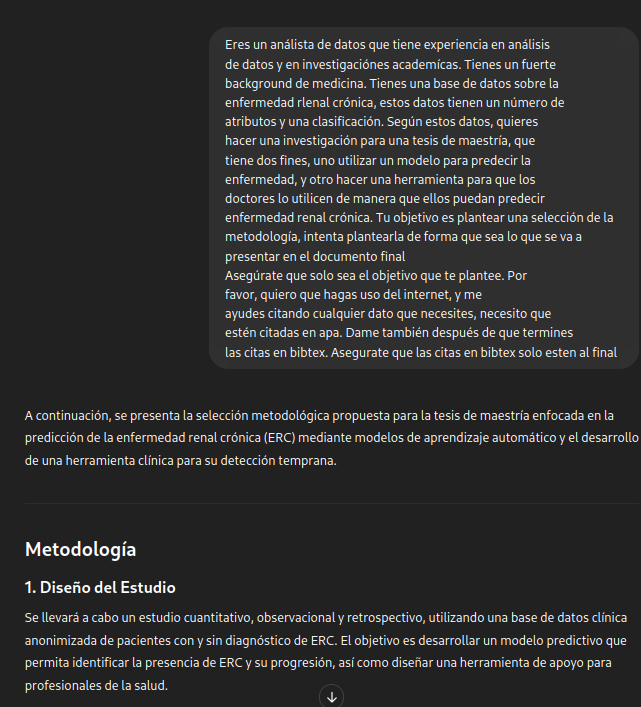
\includegraphics[width=0.6\textwidth]{../chat_1_3.png}\\
    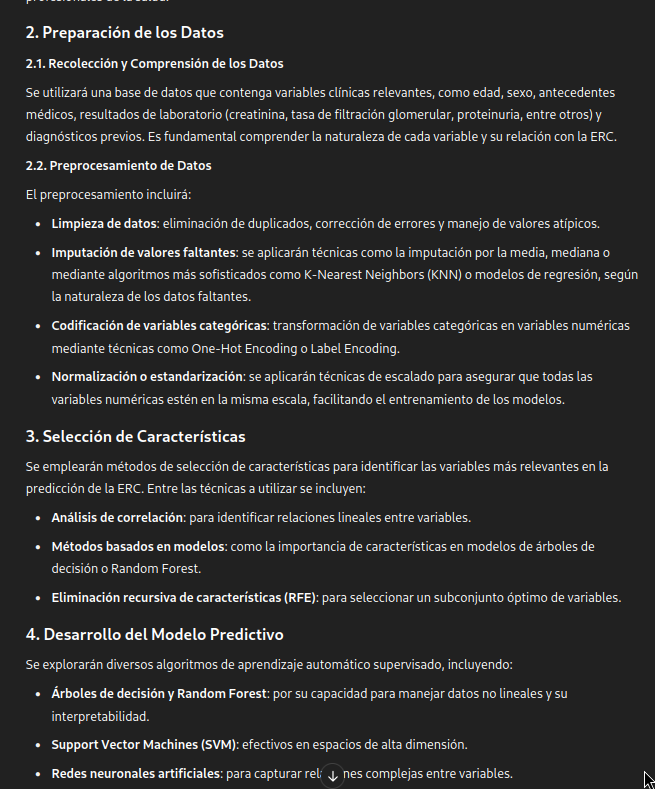
\includegraphics[width=0.6\textwidth]{../chat_2_3.png}\\
    \newpage
    \includegraphics[width=0.6\textwidth]{../chat\_3\_3.png}\\
\end{center}
\textbf{Citas encontradas por ChatGPT}
\begin{itemize}
    \item Amador Martínez, W. D. (2020). Modelos de aprendizaje automático para la predicción de la progresión de la enfermedad renal crónica. Pontificia Universidad Javeriana. Recuperado de https://repositorioslatinoamericanos.uchile.cl/handle/2250/6652473 repositorioslatinoamericanos.uchile.cl
    \item Rodríguez, J. (2019). Implementación de modelos de aprendizaje automático para la predicción de la enfermedad renal crónica. Universidad de Bogotá Jorge Tadeo Lozano. Recuperado de https://expeditiorepositorio.utadeo.edu.co/handle/20.500.12010/17638 Expedito Repositorio
    \item Li, Z., Liu, X., Tang, Z., Zhang, P., Jin, N., Eadon, M., ... \& Su, J. (2024). TrajVis: a visual clinical decision support system to translate artificial intelligence trajectory models in the precision management of chronic kidney disease. arXiv preprint arXiv:2401.08067. https://arxiv.org/abs/2401.08067 arxiv.org
    \item Jawad, K. M. T., Verma, A., Amsaad, F., \& Ashraf, L. (2024). AI-Driven Predictive Analytics Approach for Early Prognosis of Chronic Kidney Disease Using Ensemble Learning and Explainable AI. arXiv preprint arXiv:2406.06728. https://arxiv.org/abs/2406.06728 arxiv.org
    \item Ma, J., Wang, J., Lu, L., Sun, Y., Feng, M., Shen, P., ... \& Zhang, L. (2025). Development and Validation of a Dynamic Kidney Failure Prediction Model based on Deep Learning: A Real-World Study with External Validation. arXiv preprint arXiv:2501.16388.
        \\https://arxiv.org/abs/2501.16388 arxiv.org
\end{itemize}
\newpage
\subsection{Anexo 8: Resultado Gemini tercer tema}
\begin{center}
    \includegraphics[width=0.6\textwidth]{../gemini\_3.png}\\
    \includegraphics[width=0.6\textwidth]{../gemini\_2\_3.png}\\
    \includegraphics[width=0.6\textwidth]{../gemini\_3\_3.png}\\
    \includegraphics[width=0.6\textwidth]{../gemini\_4\_3.png}\\
    \includegraphics[width=0.6\textwidth]{../gemini\_5\_3.png}\\
    \includegraphics[width=0.6\textwidth]{../gemini\_6\_3.png}\\
\end{center}
\textbf{Citas encontradas por Gemini}
\begin{itemize}
    \item Breiman, L. (2001). Random Forests. Machine Learning, 45(1), 5-32.
    \item Chen, T., \& Guestrin, C. (2016). XGBoost: A Scalable Tree Boosting System. En Proceedings of the 22nd ACM SIGKDD International Conference on Knowledge Discovery and Data Mining (pp. 785-794). ACM.
    \item Chen, W., Zhang, Z., Ma, K., \& Feng, D. (2020). Ethical Issues of Using Artificial Intelligence in Healthcare: A Systematic Review. Journal of Medical Internet Research, 22(12), e18200.
    \item Cortes, C., \& Vapnik, V. (1995). Support-Vector Networks. Machine Learning, 20(3), 273-297.
\end{itemize}

\newpage
\subsection{Anexo 9: Resultado Claude tercer tema}
\begin{center}
    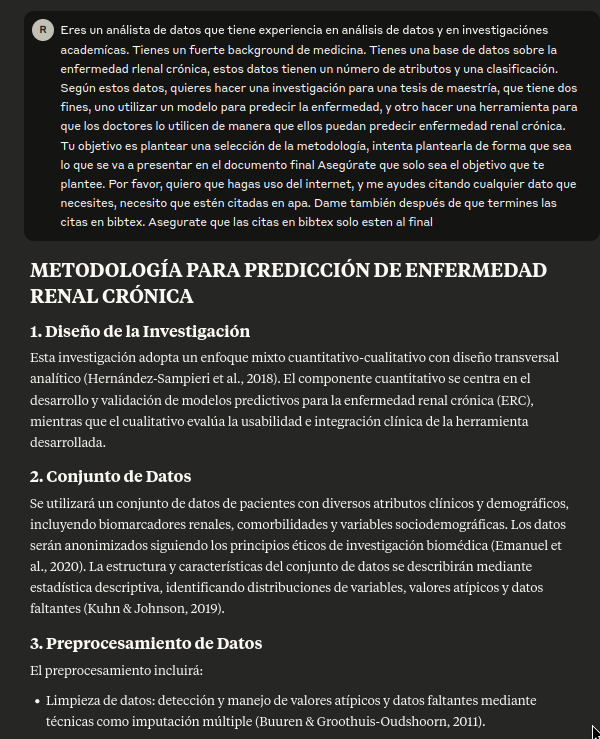
\includegraphics[width=0.6\textwidth]{../claude_1_3.png}\\
    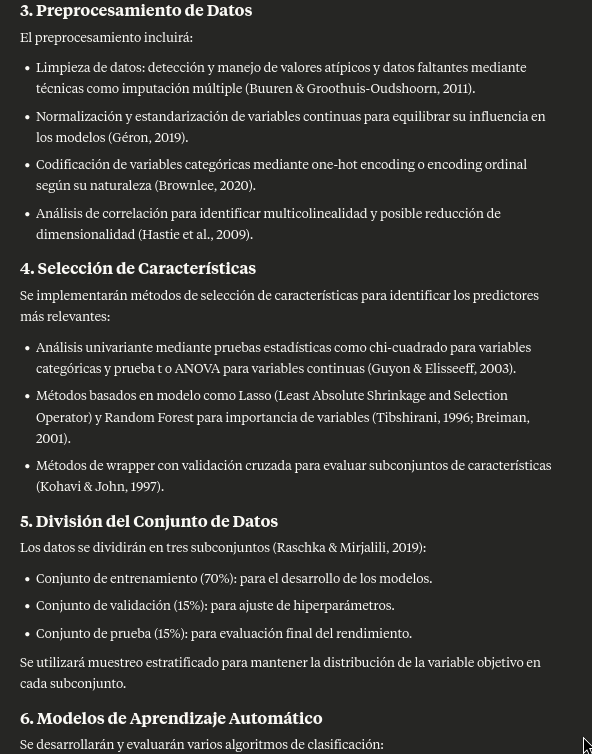
\includegraphics[width=0.6\textwidth]{../claude_2_3.png}\\
    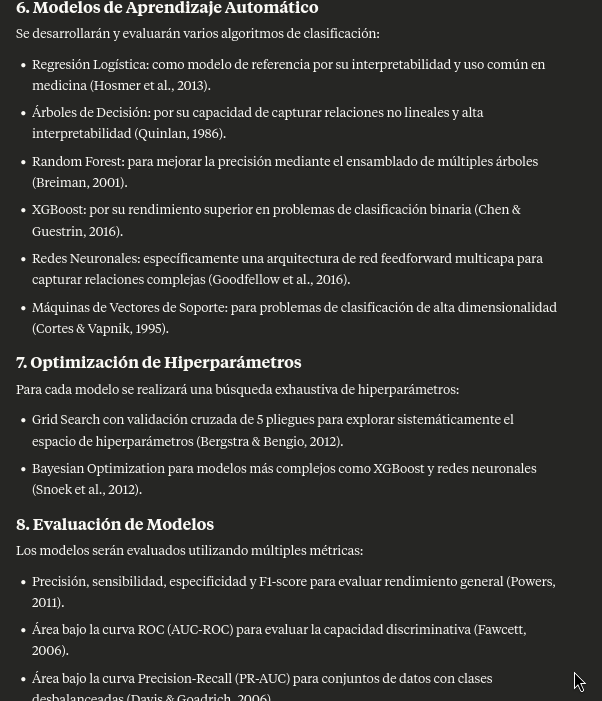
\includegraphics[width=0.6\textwidth]{../claude_3_3.png}\\
    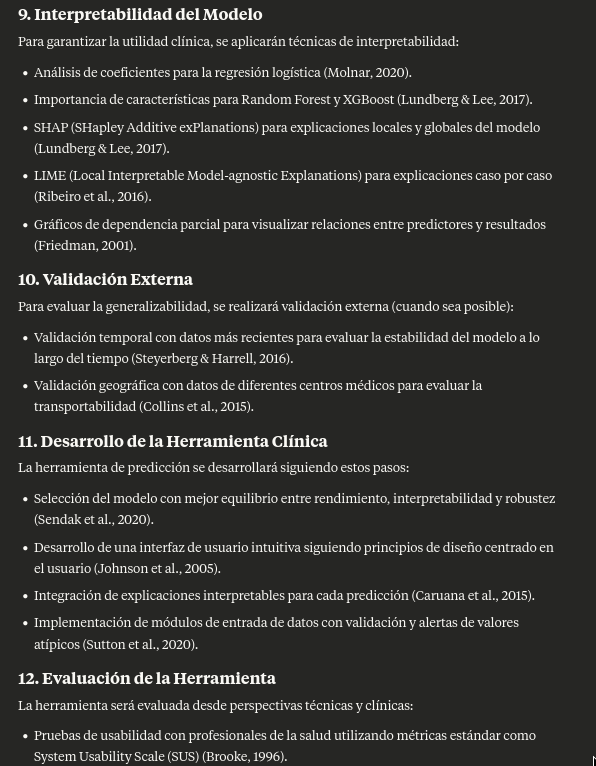
\includegraphics[width=0.6\textwidth]{../claude_5_3.png}\\
    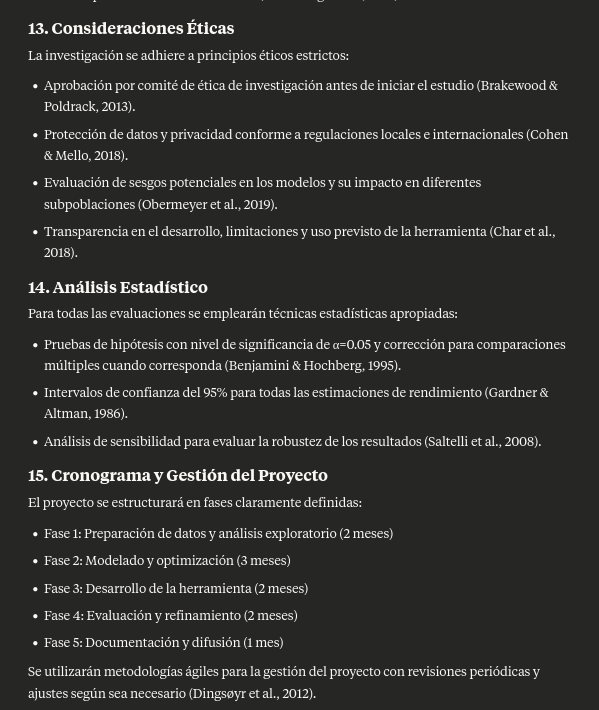
\includegraphics[width=0.6\textwidth]{../claude_6_3.png}\\
\end{center}
\newpage
\bibliographystyle{apacite}
\bibliography{main.bib}
\end{document}
